% ============================================================================
% THESIS: 1-Bit Magnitude Comparator Using GDI Technique
% Author: SHAHREAR HOSSAIN | ID: ET223104
% Supervisor: Riazul Islam, Lecturer
% Department of Electrical and Electronic Engineering
% INTERNATIONAL ISLAMIC UNIVERSITY CHITTAGONG (IIUC)
% ============================================================================

\documentclass[12pt,a4paper,oneside]{report}

% Core Packages (Universal TinyTeX / TeX Live compatibility)
\usepackage[top=1in, bottom=1in, left=1.5in, right=1in]{geometry}
\usepackage{times}
\usepackage[T1]{fontenc}
\usepackage[utf8]{inputenc}
\usepackage{graphicx}
\usepackage{amsmath,amssymb}
\usepackage{setspace}
\usepackage{array}
\usepackage{float}
\usepackage[hidelinks]{hyperref}

% Prevent report class from inserting extra blank pages before chapters
\let\cleardoublepage\clearpage

% Document Formatting
\onehalfspacing
\setlength{\parindent}{0.5in}
\setlength{\parskip}{6pt}

% Formatting Chapter Headings (IIUC Style: Centered, Bold, Uppercase)
\makeatletter
\def\@makechapterhead#1{%
  \vspace*{10\p@}%
  {\parindent \z@ \centering \normalfont
    \ifnum \c@secnumdepth >\m@ne
        \large\bfseries \MakeUppercase{\@chapapp\space \thechapter}
        \par\nobreak
        \vskip 12\p@
    \fi
    \interlinepenalty\@M
    \large \bfseries \MakeUppercase{#1}\par\nobreak
    \vskip 24\p@
  }}
\def\@makeschapterhead#1{%
  \vspace*{10\p@}%
  {\parindent \z@ \centering \normalfont
    \interlinepenalty\@M
    \large \bfseries \MakeUppercase{#1}\par\nobreak
    \vskip 24\p@
  }}
\makeatother

% Section Headings
\makeatletter
\renewcommand\section{\@startsection {section}{1}{\z@}%
                                   {-3.5ex \@plus -1ex \@minus -.2ex}%
                                   {2.3ex \@plus.2ex}%
                                   {\normalfont\normalsize\bfseries}}
\renewcommand\subsection{\@startsection{subsection}{2}{\z@}%
                                     {-3.25ex\@plus -1ex \@minus -.2ex}%
                                     {1.5ex \@plus .2ex}%
                                     {\normalfont\normalsize\bfseries\itshape}}
\renewcommand\subsubsection{\@startsection{subsubsection}{3}{\z@}%
                                     {-3.25ex\@plus -1ex \@minus -.2ex}%
                                     {1.5ex \@plus .2ex}%
                                     {\normalfont\normalsize\itshape}}
\makeatother

% Remove leader dots in Table of Contents, List of Figures, and List of Tables
\makeatletter
\renewcommand{\@dottedtocline}[5]{%
  \ifnum #1>\c@tocdepth \else
    \vskip \z@ \@plus.2\p@
    {\leftskip #2\relax \rightskip \@tocrmarg \parfillskip -\rightskip
     \parindent #2\relax\@afterindenttrue
     \interlinepenalty\@M
     \leavevmode
     \@tempdima #3\relax
     \advance\leftskip \@tempdima \null\nobreak\hskip -\leftskip
     {#4}\nobreak
     \hfill
     \nobreak\hb@xt@\@pnumwidth{\hss #5}\par}%
  \fi}
\makeatother

\graphicspath{{./}}

\begin{document}

% ========================= PAGE 1: COVER PAGE ==============================
\thispagestyle{empty}
\begin{center}
\vspace*{0.5cm}

{\large\bfseries 1-BIT MAGNITUDE COMPARATOR USING GDI TECHNIQUE}

\vspace{3cm}

by

\vspace{0.5cm}
{\normalsize SHAHREAR HOSSAIN}

\vspace{3cm}

BACHELOR OF SCIENCE\\
IN\\
ELECTRICAL AND ELECTRONIC ENGINEERING

\vspace{2.5cm}


\includegraphics[width=2.5cm]{iiuc_logo.jpg}

\vspace{1cm}

Department of Electrical and Electronic Engineering\\
INTERNATIONAL ISLAMIC UNIVERSITY CHITTAGONG

\vspace{0.5cm}
MAY 2026
\end{center}
\clearpage

% ========================= PAGE 2: INTENTIONALLY BLANK ====================
\thispagestyle{empty}
\mbox{}
\vfill
\begin{center}
\textit{This page is intentionally left blank.}
\end{center}
\vfill
\clearpage

% ========================= PAGE 3: INNER TITLE PAGE =======================
\thispagestyle{empty}
\begin{center}
\vspace*{0.5cm}

{\large\bfseries 1-BIT MAGNITUDE COMPARATOR USING GDI TECHNIQUE}

\vspace{2.5cm}

by

\vspace{0.5cm}
{\normalsize SHAHREAR HOSSAIN}

\vspace{2cm}

A thesis\\
submitted as partial fulfilment of the requirement for the degree of

\vspace{0.5cm}
BACHELOR OF SCIENCE\\
IN\\
ELECTRICAL AND ELECTRONIC ENGINEERING

\vspace{2.5cm}


\includegraphics[width=2.5cm]{iiuc_logo.jpg}

\vspace{1cm}

Department of Electrical and Electronic Engineering\\
INTERNATIONAL ISLAMIC UNIVERSITY CHITTAGONG

\vspace{0.5cm}
MAY 2026
\end{center}
\clearpage

% ========================= PAGE 4: INTENTIONALLY BLANK ====================
\thispagestyle{empty}
\mbox{}
\vfill
\begin{center}
\textit{This page is intentionally left blank.}
\end{center}
\vfill
\clearpage

% ========================= PRELIMINARY PAGES ================================
\pagenumbering{roman}
\setcounter{page}{2}

% ========================= CERTIFICATE OF APPROVAL ==========================
\chapter*{CERTIFICATE OF APPROVAL}
\addcontentsline{toc}{chapter}{CERTIFICATE OF APPROVAL}

\noindent The thesis entitled ``1-Bit Magnitude Comparator Using GDI Technique'' submitted by Shahrear Hossain, bearing Matric ID: ET223104 of the session Spring 2022, to the Department of Electrical and Electronic Engineering, International Islamic University Chittagong, has been accepted as satisfactory in partial fulfilment of the requirements for the degree of Bachelor of Science in Engineering and approved at the examination held on May 2026.

\vspace{0.6cm}

\noindent\textbf{BOARD OF EXAMINERS}

\vspace{0.8cm}

\noindent\begin{tabular}{p{6.8cm} p{6.8cm}}
\rule{6cm}{0.4pt} & \rule{6cm}{0.4pt} \\
\textbf{Supervisor} & \textbf{Examiner 1} \\
Riazul Islam & Name: \rule{4.5cm}{0.4pt} \\
Lecturer & Designation: \rule{3.5cm}{0.4pt} \\
Department of EEE, IIUC & Department of EEE, IIUC \\[1.2cm]
\rule{6cm}{0.4pt} & \rule{6cm}{0.4pt} \\
\textbf{Examiner 2} & \textbf{Head of Department} \\
Name: \rule{4.5cm}{0.4pt} & Department of EEE \\
Designation: \rule{3.5cm}{0.4pt} & International Islamic University Chittagong \\
Department of EEE, IIUC & \\
\end{tabular}

\clearpage

% ========================= DECLARATION =====================================
\chapter*{DECLARATION}
\addcontentsline{toc}{chapter}{DECLARATION}

\noindent We hereby declare that this thesis/project report is the result of my/our own independent work and that no part of this work has been submitted elsewhere for the award of any degree or diploma. This work does not include any contribution from collaborative work, except where explicitly stated in the text.

\vspace{0.15cm}
\noindent We further declare that:

\vspace{0.15cm}
\noindent\textbf{\textit{Originality and Plagiarism}}\\
This report is an original work. All sources of information, ideas, and data have been properly acknowledged and referenced in accordance with the guidelines of the Department of Electrical and Electronic Engineering (EEE), International Islamic University Chittagong (IIUC).

\vspace{0.15cm}
\noindent\textbf{\textit{Data Integrity}}\\
The data presented in this report are genuine, and have been collected, processed, analyzed, and reported with academic honesty. No data have been fabricated, falsified, or manipulated in any form to influence the results or conclusions.

\vspace{0.15cm}
\noindent\textbf{\textit{Human/Animal Subjects}} \textit{(select as applicable)}\\
$\square$ This research did not involve human or animal subjects.\\
$\square$ This research involving human participants was conducted with prior ethical approval from the relevant authority. Informed consent was obtained from all participants, and their confidentiality has been strictly maintained.

\vspace{0.15cm}
\noindent\textbf{\textit{Conflict of Interest}}\\
The authors declare that there is no conflict of interest that could have influenced the conduct, analysis, or interpretation of this study.

\vspace{0.15cm}
\noindent\textbf{\textit{Ethical Compliance}}\\
This work has been carried out in accordance with the research ethics guidelines instructed by the department.

\vspace{0.4cm}

\noindent\begin{tabular}{|>{\centering\arraybackslash}p{6.8cm}|>{\centering\arraybackslash}p{6.8cm}|}
\hline
\textbf{Name of the Students} & \textbf{Signature of the Students} \\
\hline
\rule{0pt}{1.0cm} Shahrear Hossain & \rule{0pt}{1.0cm} \\[0.3cm]
\hline
\end{tabular}

\clearpage

% ========================= DEDICATION ======================================
\chapter*{DEDICATION}
\addcontentsline{toc}{chapter}{DEDICATION}

\vspace*{3cm}
\begin{center}
\textit{This thesis is dedicated to my beloved parents,\\
whose unconditional love, endless sacrifices,\\
and unwavering faith in my abilities\\
have been the greatest source of my inspiration.\\[1cm]
And to the Almighty Allah,\\
for bestowing upon me the strength and wisdom\\
to accomplish this work.}
\end{center}

\clearpage

% ========================= ACKNOWLEDGMENT ==================================
\chapter*{ACKNOWLEDGEMENT}
\addcontentsline{toc}{chapter}{ACKNOWLEDGEMENT}

\noindent All praises and thanks to Allah, the Lord of the world, the most Beneficent, the most Merciful for helping us to accomplish this work.

\vspace{0.4cm}
\noindent We are beholden to a number of people, who supported us to carry out this work for this we thank our supervisor, \textbf{Riazul Islam} who with his undying support helped us accomplish lot of hard work and to him we are grateful. Whose guidance was invaluable to us in our journey of writing this thesis. Secondly, we would also like to thank our family and our senior colleague who have helped us achieve our goal. They help us in realizing our potential as engineers and are always supporting us in our pursuit of excellence.

\vspace{1.5cm}
\noindent Authors

\clearpage

% ========================= ABSTRACT ========================================
\chapter*{ABSTRACT}
\addcontentsline{toc}{chapter}{ABSTRACT}

\noindent The rapid expansion of mobile computing, wearable electronics, implantable biomedical devices, wireless sensor networks, and edge computing architectures has elevated power minimization to a paramount design objective in modern Very Large Scale Integration (VLSI) systems. Among the foundational building blocks of digital computing architectures, digital magnitude comparators play an indispensable role in arithmetic logic units (ALUs), central processing units (CPUs), digital signal processors (DSPs), data sorting engines, and high-speed flash analog-to-digital converters (ADCs). Conventional digital comparators implemented using standard static Complementary Metal-Oxide-Semiconductor (CMOS) logic provide robust noise margins, stable full-rail output voltage swing, and reliable switching characteristics; however, they require a high transistor count (typically 32 transistors for a 1-bit magnitude comparator), resulting in elevated active and leakage power dissipation, large parasitic interconnect capacitance, and increased silicon footprint.

\noindent To overcome these intrinsic limitations, this thesis presents the comprehensive design, transistor-level implementation, and multi-parameter performance analysis of an ultra-low-power, high-speed 1-bit magnitude comparator based on the Gate Diffusion Input (GDI) technique. The GDI methodology represents an effective low-power circuit design paradigm that permits the realization of complex logic functions with a substantially reduced transistor count compared to conventional CMOS and pass-transistor implementations. The proposed GDI-based 1-bit comparator circuit accomplishes the generation of all three arithmetic comparison outputs ($A>B$, $A=B$, and $A<B$) using only 10 transistors (5 NMOS and 5 PMOS), achieving a remarkable 68.75\% reduction in transistor count over the standard 32-transistor static CMOS design.

\noindent The proposed circuit, along with conventional static CMOS, Transmission Gate Logic (TGL), and Pass Transistor Logic (PTL) comparator benchmarks, has been modeled and rigorously evaluated using LTSpice with the Predictive Technology Model (PTM) at the 180nm CMOS technology node under a supply voltage of 1.8V. The simulation results confirm complete functional correctness across all four possible input combinations. Extensive quantitative evaluations reveal that the proposed GDI comparator achieves an exceptionally low average power dissipation of 34.18~pW, representing a 73.83\% power reduction compared to static CMOS (130.61~pW) and a 10.34\% reduction compared to PTL (38.12~pW). Furthermore, the proposed design achieves a minimum propagation delay of 336~ps for the equality ($A=B$) output, outperforming static CMOS (398.09~ps), transmission gate (587.24~ps), and pass transistor (421.77~ps) designs by 15.59\%, 42.78\%, and 20.33\%, respectively. The resulting Power-Delay Product (PDP) of 0.0000114~fJ confirms that the proposed GDI comparator achieves the highest energy efficiency per switching operation among all evaluated configurations. Extended multi-node scaling investigations across 180nm, 90nm, and 45nm technology regimes demonstrate sustained performance scalability. This research delivers an area-efficient, low-power digital comparator suitable for next-generation energy-constrained VLSI applications.

\clearpage

% ========================= TABLE OF CONTENTS ================================
\tableofcontents
\clearpage

% ========================= LIST OF FIGURES =================================
\listoffigures
\clearpage

% ========================= LIST OF TABLES ==================================
\listoftables
\clearpage

% ========================= LIST OF ABBREVIATIONS ===========================
\chapter*{LIST OF ABBREVIATIONS}
\addcontentsline{toc}{chapter}{LIST OF ABBREVIATIONS}

\noindent\begin{tabular}{p{3cm} p{10.5cm}}
\textbf{ADC} & Analog-to-Digital Converter \\[5pt]
\textbf{ALU} & Arithmetic Logic Unit \\[5pt]
\textbf{ASIC} & Application-Specific Integrated Circuit \\[5pt]
\textbf{BJT} & Bipolar Junction Transistor \\[5pt]
\textbf{BSIM} & Berkeley Short-channel IGFET Model \\[5pt]
\textbf{C-CMOS} & Conventional Complementary Metal-Oxide-Semiconductor \\[5pt]
\textbf{CAM} & Content-Addressable Memory \\[5pt]
\textbf{CMOS} & Complementary Metal-Oxide-Semiconductor \\[5pt]
\textbf{CPU} & Central Processing Unit \\[5pt]
\textbf{DIBL} & Drain-Induced Barrier Lowering \\[5pt]
\textbf{DSP} & Digital Signal Processor \\[5pt]
\textbf{EDP} & Energy-Delay Product \\[5pt]
\textbf{ENOB} & Effective Number of Bits \\[5pt]
\textbf{FDSOI} & Fully Depleted Silicon-on-Insulator \\[5pt]
\textbf{FinFET} & Fin Field-Effect Transistor \\[5pt]
\textbf{FOM} & Figure of Merit \\[5pt]
\textbf{FPGA} & Field-Programmable Gate Array \\[5pt]
\textbf{GAA} & Gate-All-Around \\[5pt]
\textbf{GDI} & Gate Diffusion Input \\[5pt]
\textbf{GIDL} & Gate-Induced Drain Leakage \\[5pt]
\textbf{HCI} & Hot-Carrier Injection \\[5pt]
\textbf{IC} & Integrated Circuit \\[5pt]
\textbf{IoT} & Internet of Things \\[5pt]
\textbf{IRDS} & International Roadmap for Devices and Systems \\[5pt]
\textbf{ITRS} & International Technology Roadmap for Semiconductors \\[5pt]
\textbf{K-map} & Karnaugh Map \\[5pt]
\textbf{MOSFET} & Metal-Oxide-Semiconductor Field-Effect Transistor \\[5pt]
\textbf{MTCMOS} & Multi-Threshold Complementary Metal-Oxide-Semiconductor \\[5pt]
\textbf{MUX} & Multiplexer \\[5pt]
\textbf{NBTI} & Negative-Bias Temperature Instability \\[5pt]
\textbf{NMOS} & N-channel Metal-Oxide-Semiconductor \\[5pt]
\textbf{PDP} & Power-Delay Product \\[5pt]
\textbf{PMOS} & P-channel Metal-Oxide-Semiconductor \\[5pt]
\textbf{PTL} & Pass Transistor Logic \\[5pt]
\textbf{PTM} & Predictive Technology Model \\[5pt]
\textbf{PVT} & Process, Voltage, and Temperature \\[5pt]
\textbf{SCE} & Short-Channel Effects \\[5pt]
\textbf{SNM} & Static Noise Margin \\[5pt]
\textbf{SOC} & System on Chip \\[5pt]
\textbf{SOP} & Sum of Products \\[5pt]
\textbf{SPICE} & Simulation Program with Integrated Circuit Emphasis \\[5pt]
\textbf{SSI} & Small-Scale Integration \\[5pt]
\textbf{TDDB} & Time-Dependent Dielectric Breakdown \\[5pt]
\textbf{TG / TGL} & Transmission Gate / Transmission Gate Logic \\[5pt]
\textbf{TLB} & Translation Lookaside Buffer \\[5pt]
\textbf{TSMC} & Taiwan Semiconductor Manufacturing Company \\[5pt]
\textbf{ULSI} & Ultra Large Scale Integration \\[5pt]
\textbf{VLSI} & Very Large Scale Integration \\[5pt]
\textbf{VTC} & Voltage Transfer Characteristic \\[5pt]
\textbf{XNOR} & Exclusive-NOR Logic Gate \\[5pt]
\textbf{XOR} & Exclusive-OR Logic Gate \\
\end{tabular}

\clearpage

% ========================= LIST OF SYMBOLS =================================
\chapter*{LIST OF SYMBOLS}
\addcontentsline{toc}{chapter}{LIST OF SYMBOLS}

\noindent\begin{tabular}{p{3cm} p{10.5cm}}
$V_{DD}$ & Supply voltage \\[5pt]
$V_{th}$ & Threshold voltage \\[5pt]
$V_{th0}$ & Zero-bias threshold voltage \\[5pt]
$V_{thn}$ & NMOS threshold voltage \\[5pt]
$V_{thp}$ & PMOS threshold voltage \\[5pt]
$V_{gs}$ & Gate-to-source voltage \\[5pt]
$V_{ds}$ & Drain-to-source voltage \\[5pt]
$V_{sb}$ & Source-to-body (substrate) voltage \\[5pt]
$V_{OH}$ & Output high voltage \\[5pt]
$V_{OL}$ & Output low voltage \\[5pt]
$V_{IH}$ & Input high voltage \\[5pt]
$V_{IL}$ & Input low voltage \\[5pt]
$I_{ds}$ & Drain-to-source current \\[5pt]
$I_{sub}$ & Subthreshold leakage current \\[5pt]
$I_{gate}$ & Gate tunneling leakage current \\[5pt]
$C_{ox}$ & Gate oxide capacitance per unit area \\[5pt]
$C_{load}$ & Total output load capacitance \\[5pt]
$t_{ox}$ & Gate oxide thickness \\[5pt]
$W$ & Channel width \\[5pt]
$L$ & Channel length \\[5pt]
$W/L$ & Transistor aspect ratio \\[5pt]
$\mu_n$ & Electron mobility \\[5pt]
$\mu_p$ & Hole mobility \\[5pt]
$\beta_n$ & NMOS transconductance parameter \\[5pt]
$\beta_p$ & PMOS transconductance parameter \\[5pt]
$\alpha_{0\rightarrow 1}$ & Switching activity factor \\[5pt]
$f$ & Operating frequency \\[5pt]
$t_r$ & Rise time (10\% to 90\%) \\[5pt]
$t_f$ & Fall time (90\% to 10\%) \\[5pt]
$t_{pd}$ & Propagation delay \\[5pt]
$t_{pHL}$ & High-to-low propagation delay \\[5pt]
$t_{pLH}$ & Low-to-high propagation delay \\[5pt]
$P_{avg}$ & Average power dissipation \\[5pt]
$P_{dyn}$ & Dynamic switching power \\[5pt]
$P_{sc}$ & Short-circuit power \\[5pt]
$P_{stat}$ & Static (leakage) power \\[5pt]
$v_T$ & Thermal voltage ($kT/q$) \\[5pt]
$k_B$ & Boltzmann constant ($1.38 \times 10^{-23}$ J/K) \\[5pt]
$q$ & Electron charge ($1.6 \times 10^{-19}$ C) \\[5pt]
$T$ & Absolute temperature \\[5pt]
$\gamma$ & Body-effect coefficient \\[5pt]
$\phi_F$ & Fermi potential \\[5pt]
$\eta$ & DIBL coefficient \\[5pt]
$\kappa$ & Scaling factor \\
\end{tabular}

\clearpage

% ========================= MAIN BODY =======================================
\pagenumbering{arabic}
\setcounter{page}{1}

% ############################################################################
% CHAPTER 1: INTRODUCTION
% ############################################################################
\chapter{INTRODUCTION}

\section{Background and Context}

The modern world is built upon a vast and ever-expanding infrastructure of electronic systems. From the smartphones in our pockets to the supercomputers driving artificial intelligence research, digital electronic circuits form the backbone of contemporary computing, communication, and control systems. The relentless drive toward higher computational performance, lower power consumption, and more compact form factors has been the defining force in the semiconductor industry for over half a century. As electronic devices continue to permeate every aspect of human activity—including healthcare, transportation, industrial automation, environmental monitoring, and entertainment—the demand for energy-efficient digital circuits has never been greater.

At the heart of every digital computing system lies a collection of fundamental building blocks: logic gates, arithmetic units, memory elements, and comparators. Among these, the digital magnitude comparator stands as one of the most frequently instantiated combinational circuits in modern processor architectures. A magnitude comparator evaluates the relative arithmetic values of two binary inputs and generates output signals indicating whether one input is greater than, equal to, or less than the other. This seemingly simple operation underpins critical functions in microprocessors, digital signal processors, data sorting networks, analog-to-digital converters, and cache memory systems.

Given the ubiquity of comparators in digital systems, even modest improvements in their power consumption, propagation delay, or silicon area can yield substantial cumulative benefits when scaled across billions of transistors in a modern integrated circuit. This thesis addresses this challenge by proposing and evaluating an optimized 1-bit magnitude comparator based on the Gate Diffusion Input (GDI) technique, a low-power design methodology that achieves complex logic functions with minimal transistor count.

\section{Historical Evolution of Semiconductor Technology}

The microelectronics and semiconductor industries have undergone unprecedented expansion over the last several decades, driven largely by the continuous dimensional scaling of silicon Field-Effect Transistors. The journey of solid-state electronics began with the invention of the point-contact transistor by John Bardeen, Walter Brattain, and William Shockley at Bell Laboratories in 1947, which replaced bulky, power-hungry vacuum tubes and initiated the modern electronic era. The subsequent realization of monolithic integrated circuits by Jack Kilby and Robert Noyce in the late 1950s paved the way for placing multiple interconnected components on a single semiconductor substrate.

In 1965, Gordon Moore formulated the empirical observation that the number of transistors on a microchip doubles approximately every two years, an observation that became the technological roadmap for the semiconductor industry known as Moore's Law [1]. Figure~\ref{fig:moores_law} illustrates this remarkable trajectory, showing the exponential growth in transistor density from the Intel 4004 processor in 1971 to modern multi-billion-transistor system-on-chip designs.

\begin{figure}[H]
\centering
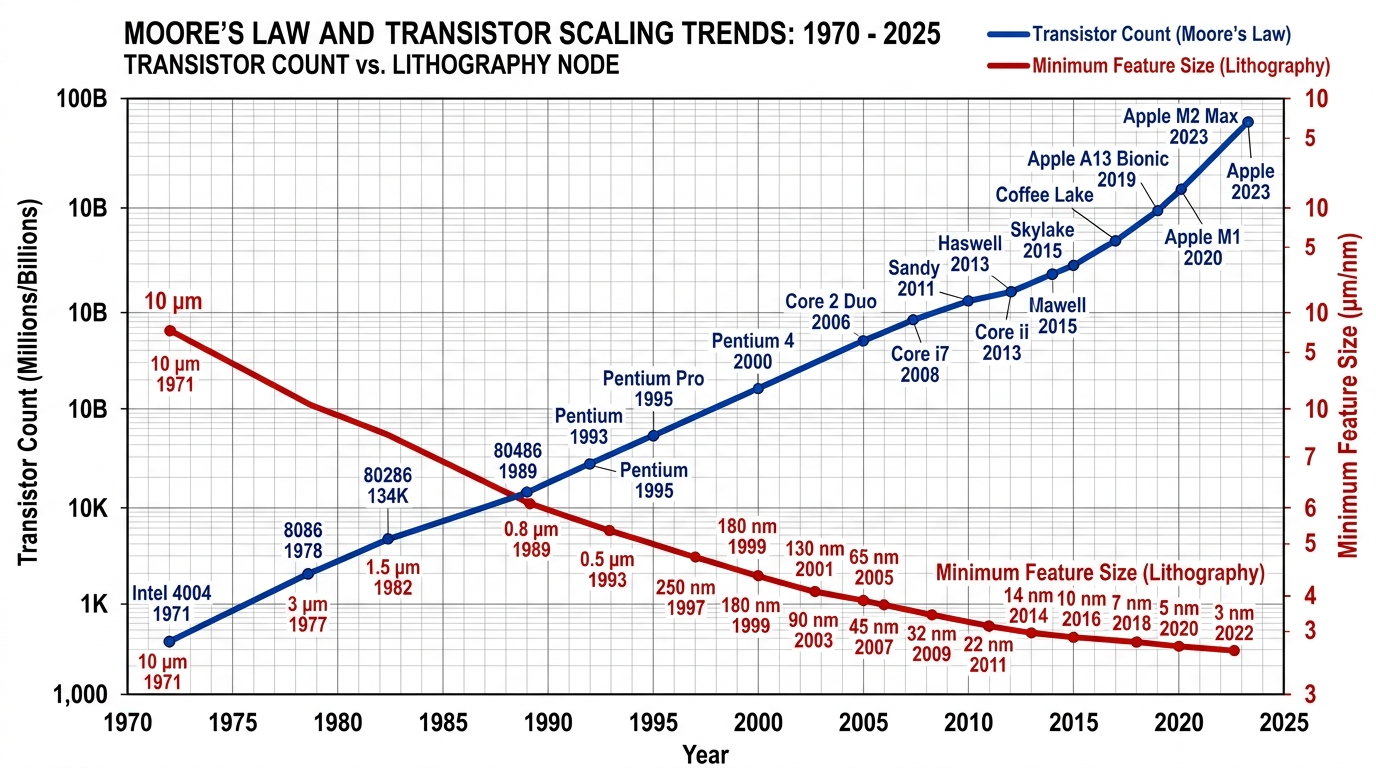
\includegraphics[width=0.95\textwidth]{moores_law_scaling.jpg}
\caption{Moore's Law: Historical trend of transistor count growth and minimum feature size reduction in semiconductor technology from 1970 to 2025.}
\label{fig:moores_law}
\end{figure}

In 1974, Robert Dennard established the principles of constant electric-field scaling, demonstrating that as MOSFET physical dimensions (gate length $L$, gate width $W$, and gate oxide thickness $t_{ox}$) are scaled down by a factor $\kappa > 1$, the supply voltage $V_{DD}$ and threshold voltage $V_{th}$ can also be scaled by $1/\kappa$. This proportional scaling maintained a constant electric field across the gate dielectric, resulting in circuits that operated faster by a factor $\kappa$, consumed $1/\kappa^2$ less power per device, and exhibited constant power density per unit silicon area [2].

The key relationships governing Dennard scaling are summarized in Table~\ref{tab:dennard_scaling}.

\begin{table}[H]
\centering
\caption{Dennard's constant electric-field scaling relationships for MOSFET devices.}
\label{tab:dennard_scaling}
\vspace{0.2cm}
\begin{tabular}{|l|c|c|}
\hline
\textbf{Device/Circuit Parameter} & \textbf{Scaling Factor} & \textbf{Effect} \\
\hline
Gate length ($L$) & $1/\kappa$ & Smaller device \\
\hline
Gate width ($W$) & $1/\kappa$ & Smaller device \\
\hline
Gate oxide thickness ($t_{ox}$) & $1/\kappa$ & Thinner dielectric \\
\hline
Supply voltage ($V_{DD}$) & $1/\kappa$ & Lower voltage \\
\hline
Threshold voltage ($V_{th}$) & $1/\kappa$ & Lower threshold \\
\hline
Current density ($J$) & $\kappa$ & Higher current per area \\
\hline
Gate delay ($t_{pd}$) & $1/\kappa$ & Faster switching \\
\hline
Power per device ($P$) & $1/\kappa^2$ & Lower power \\
\hline
Power density ($P/A$) & $1$ & Constant \\
\hline
\end{tabular}
\end{table}

Thanks to Dennard scaling, integrated circuits progressed rapidly from Small-Scale Integration (SSI) with tens of transistors to Very Large Scale Integration (VLSI) and Ultra Large Scale Integration (ULSI) architectures integrating billions of complementary metal-oxide-semiconductor (CMOS) devices on a single monolithic die [3]. Modern system-on-chip (SoC) platforms now execute trillions of instructions per second, powering applications from cloud supercomputers to handheld smart devices.

\section{MOSFET Device Physics Fundamentals}

The Metal-Oxide-Semiconductor Field-Effect Transistor (MOSFET) is the fundamental building block of all modern digital integrated circuits. Understanding its operating principles is essential for appreciating the design trade-offs involved in comparator circuit optimization. Figure~\ref{fig:mosfet_cross} presents the cross-sectional view of both NMOS and PMOS transistor structures on a silicon substrate.

\begin{figure}[H]
\centering
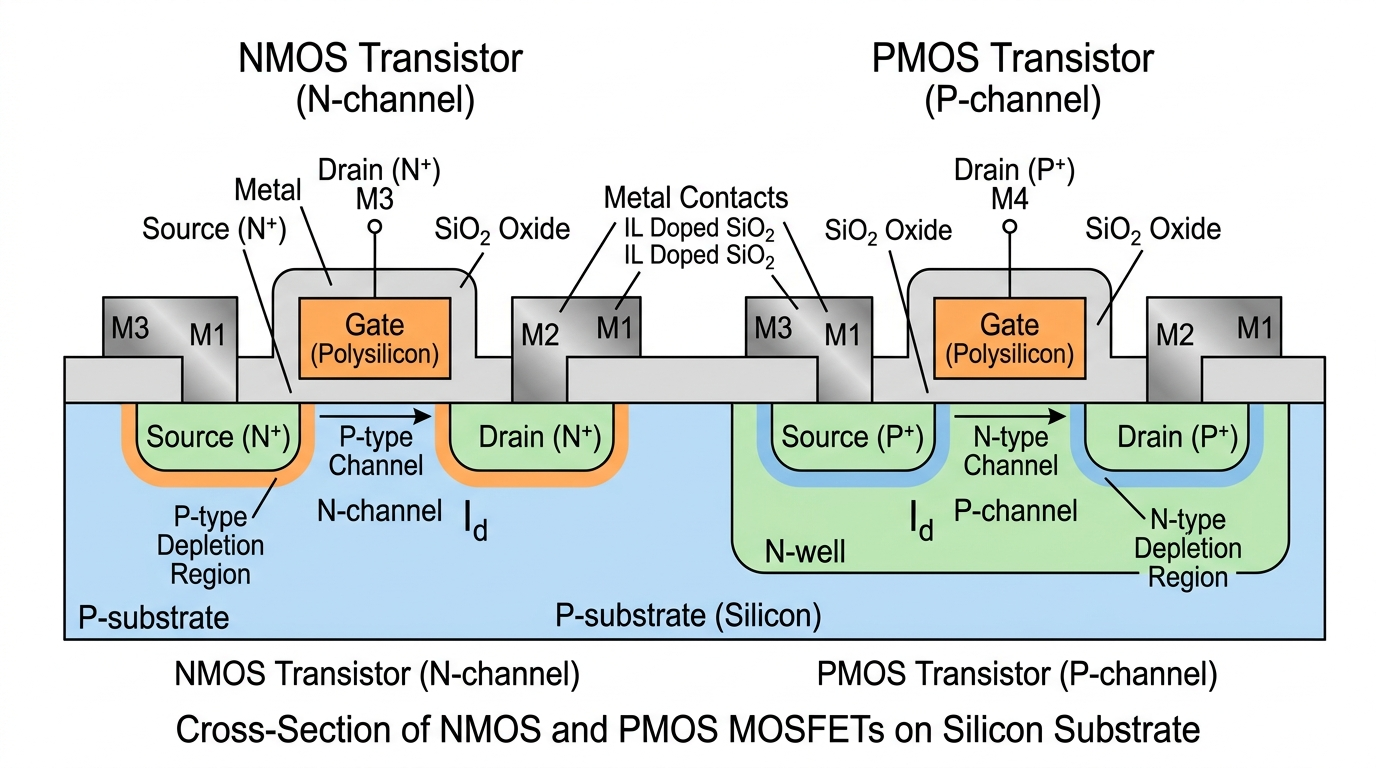
\includegraphics[width=0.95\textwidth]{mosfet_cross_section.jpg}
\caption{Cross-sectional diagram of NMOS (N-channel) and PMOS (P-channel) MOSFET transistors fabricated on a common P-type silicon substrate, showing gate, source, drain, gate oxide, channel, and well regions.}
\label{fig:mosfet_cross}
\end{figure}

\subsection{MOSFET Operating Regions}

An NMOS transistor operates in three distinct regions, depending on the terminal voltages:

\noindent\textbf{1. Cutoff Region ($V_{gs} < V_{th}$):} The transistor is nominally ``OFF.'' No inversion layer exists under the gate, and the drain current is ideally zero. In practice, a small subthreshold leakage current flows, which becomes significant in nanometer-scale devices.

\noindent\textbf{2. Linear (Triode) Region ($V_{gs} > V_{th}$ and $V_{ds} < V_{gs} - V_{th}$):} The transistor operates as a voltage-controlled resistor. The drain current is given by:
\begin{equation}
I_{ds} = \mu_n C_{ox} \frac{W}{L} \left[(V_{gs} - V_{th})V_{ds} - \frac{V_{ds}^2}{2}\right]
\label{eq:ids_linear}
\end{equation}

\noindent\textbf{3. Saturation Region ($V_{gs} > V_{th}$ and $V_{ds} \geq V_{gs} - V_{th}$):} The channel is pinched off at the drain end. The drain current becomes relatively independent of $V_{ds}$ and is governed by:
\begin{equation}
I_{ds} = \frac{1}{2} \mu_n C_{ox} \frac{W}{L} (V_{gs} - V_{th})^2 (1 + \lambda V_{ds})
\label{eq:ids_sat}
\end{equation}
where $\lambda$ is the channel-length modulation parameter.

For PMOS transistors, the operating equations are analogous but with reversed voltage polarities and hole mobility $\mu_p$ replacing electron mobility $\mu_n$.

\subsection{Threshold Voltage and Body Effect}

The threshold voltage $V_{th}$ is a critical parameter that determines the gate voltage required to form an inversion layer and turn the transistor ON. For an NMOS transistor, the zero-bias threshold voltage is given by:
\begin{equation}
V_{th0} = V_{FB} + 2\phi_F + \frac{\sqrt{2 q \epsilon_{si} N_A (2\phi_F)}}{C_{ox}}
\label{eq:vth0}
\end{equation}
where $V_{FB}$ is the flat-band voltage, $\phi_F = (kT/q) \ln(N_A/n_i)$ is the Fermi potential, $\epsilon_{si}$ is the silicon permittivity, $N_A$ is the substrate doping concentration, and $n_i$ is the intrinsic carrier concentration.

When the source terminal is not at the same potential as the substrate (body), the body effect causes the threshold voltage to increase:
\begin{equation}
V_{th} = V_{th0} + \gamma \left(\sqrt{2\phi_F + V_{sb}} - \sqrt{2\phi_F}\right)
\label{eq:bodyeffect}
\end{equation}
where $\gamma = \sqrt{2 q \epsilon_{si} N_A}/C_{ox}$ is the body-effect coefficient and $V_{sb}$ is the source-to-body voltage. This effect is particularly important in Pass Transistor Logic (PTL) and Gate Diffusion Input (GDI) circuits, where transistor source terminals are not always connected to fixed supply rails.

\subsection{CMOS Inverter: The Fundamental Logic Gate}

The CMOS inverter represents the most fundamental logic gate in complementary MOS technology. It consists of a PMOS transistor (pull-up network) connected in series with an NMOS transistor (pull-down network), with their gates connected together as the input and their drains connected together as the output. Figure~\ref{fig:cmos_inverter} illustrates the CMOS inverter circuit schematic and its corresponding Voltage Transfer Characteristic (VTC).

\begin{figure}[H]
\centering
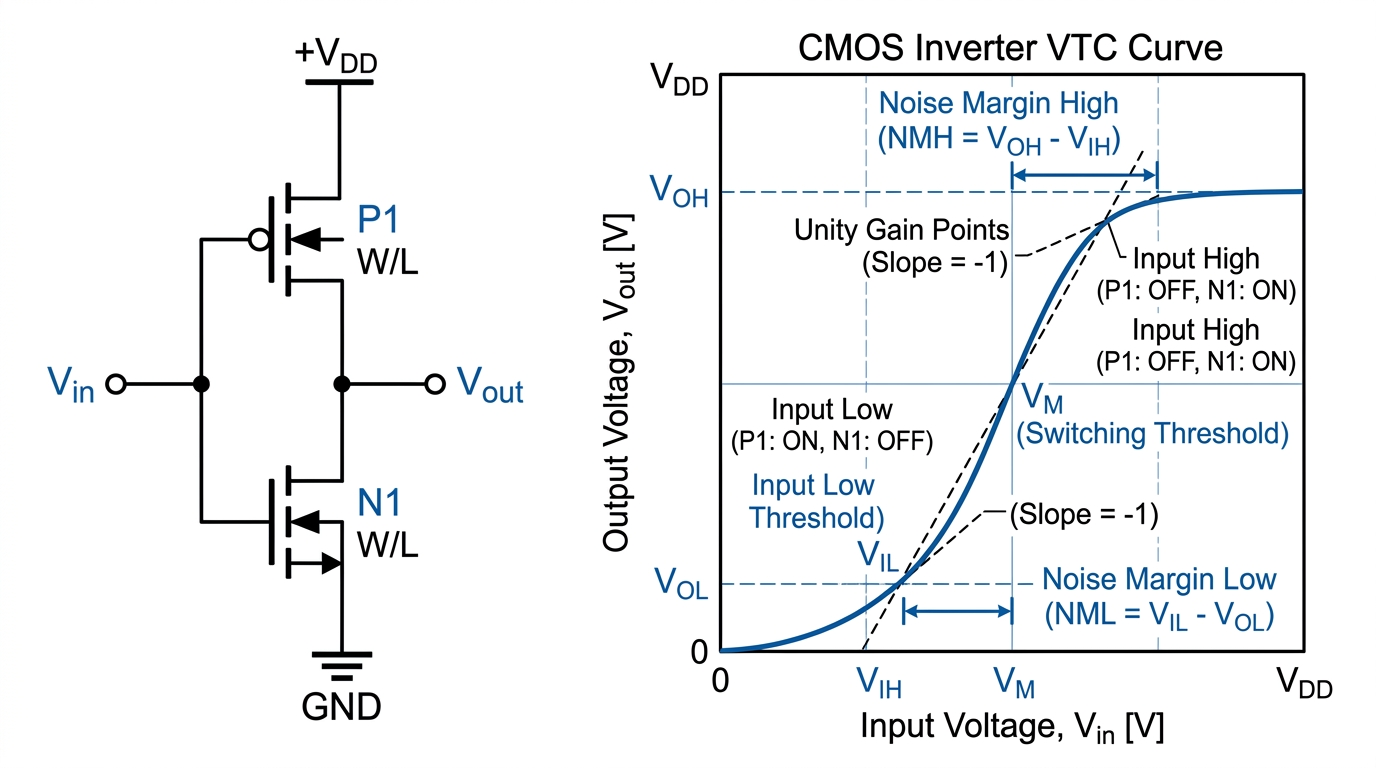
\includegraphics[width=0.95\textwidth]{cmos_inverter_vtc.jpg}
\caption{CMOS inverter: (left) transistor-level circuit schematic showing PMOS pull-up and NMOS pull-down configuration; (right) voltage transfer characteristic (VTC) curve with labeled noise margin parameters $V_{OH}$, $V_{OL}$, $V_{IH}$, $V_{IL}$, and switching threshold $V_M$.}
\label{fig:cmos_inverter}
\end{figure}

The VTC of a CMOS inverter exhibits several important characteristics that define the quality of the logic gate:
\begin{itemize}
\item \textbf{Output High Voltage ($V_{OH}$):} Ideally equal to $V_{DD}$, representing full rail-to-rail output swing.
\item \textbf{Output Low Voltage ($V_{OL}$):} Ideally equal to $0\text{V}$ (ground).
\item \textbf{Noise Margin High ($NM_H$):} $NM_H = V_{OH} - V_{IH}$, representing the tolerance to noise on a logic-high signal.
\item \textbf{Noise Margin Low ($NM_L$):} $NM_L = V_{IL} - V_{OL}$, representing the tolerance to noise on a logic-low signal.
\item \textbf{Switching Threshold ($V_M$):} The input voltage at which the output voltage equals the input voltage ($V_{out} = V_{in}$), which ideally occurs at $V_{DD}/2$ for symmetric transistor sizing.
\end{itemize}

The switching threshold can be computed as:
\begin{equation}
V_M = \frac{V_{DD} + V_{thp} + V_{thn}\sqrt{\beta_n/\beta_p}}{1 + \sqrt{\beta_n/\beta_p}}
\label{eq:switching_threshold}
\end{equation}

For balanced switching ($V_M = V_{DD}/2$), the PMOS width must be made larger than the NMOS width to compensate for the lower hole mobility, typically by a ratio of $W_p/W_n \approx \mu_n/\mu_p \approx 2.0$ to $2.5$.

\section{Nanoscale Scaling Limits and the Low-Power Imperative}

However, as transistor physical gate lengths scaled deep into the sub-micron and nanometer regimes (below 180nm), classical Dennardian scaling reached its fundamental physical limits. The primary roadblock arose from the inability to scale the threshold voltage $V_{th}$ proportionally with $V_{DD}$ without causing an exponential increase in subthreshold leakage currents. In silicon MOSFETs, subthreshold current is governed by the Boltzmann thermodynamic distribution of electron energies, which imposes an invariant physical limit on the subthreshold swing of approximately $60\text{ mV/decade}$ at room temperature ($300\text{ K}$). Consequently, reducing $V_{th}$ to preserve gate overdrive $(V_{DD} - V_{th})$ at lower supply voltages leads to unacceptable static leakage currents when transistors are in the nominal ``OFF'' state [12].

As a consequence of the breakdown of Dennard scaling, modern microprocessors can no longer operate all integrated transistors simultaneously at maximum clock frequency without exceeding thermal dissipation limits. This physical barrier, widely known as the ``Power Wall'' and the phenomenon of ``Dark Silicon,'' has firmly established power dissipation as the central design constraint in contemporary VLSI engineering [3].

In modern electronic systems, power consumption constraints manifest across multiple operating domains:
\begin{enumerate}
\item \textbf{Battery-Operated and Portable Devices:} For smartphones, wearable health monitors, tablet computers, and remote sensor nodes, battery operating life is directly governed by total circuit power dissipation. Frequent recharging or battery replacement is often impractical, making microwatt and picowatt circuit design essential [1].
\item \textbf{High-Performance Computing and Data Centers:} In high-density server farms and supercomputers, excessive power dissipation generates severe localized heat (hot spots), requiring complex liquid-cooling systems, escalating operational electricity costs, and reducing overall system reliability [4].
\item \textbf{Device Reliability and Silicon Lifetime:} Elevated operating temperatures accelerate destructive physical failure mechanisms, including electromigration in metal interconnects, Time-Dependent Dielectric Breakdown (TDDB) in gate oxides, Negative-Bias Temperature Instability (NBTI) in PMOS devices, and Hot-Carrier Injection (HCI) in NMOS devices [7].
\item \textbf{Internet of Things (IoT) and Edge Computing:} Billions of IoT sensor nodes deployed in smart cities, industrial monitoring, and precision agriculture require ultra-low-power operation to function autonomously for years without battery replacement or external power sources.
\item \textbf{Biomedical and Implantable Devices:} Implantable cardiac pacemakers, cochlear implants, and neural recording interfaces must operate for extended periods (5 to 10 years) on small batteries, making every picojoule of energy critical for patient safety and device longevity.
\end{enumerate}

To address these challenges, circuit designers must implement energy-efficient logic structures and optimize fundamental digital building blocks.

\section{Overview of VLSI Design Flow}

The design of modern integrated circuits follows a systematic top-down methodology that progresses from abstract system specifications to physical silicon layout. Understanding this design flow provides important context for appreciating where transistor-level circuit optimization fits within the broader engineering workflow. Figure~\ref{fig:vlsi_flow} illustrates the standard VLSI IC design flow.

\begin{figure}[H]
\centering
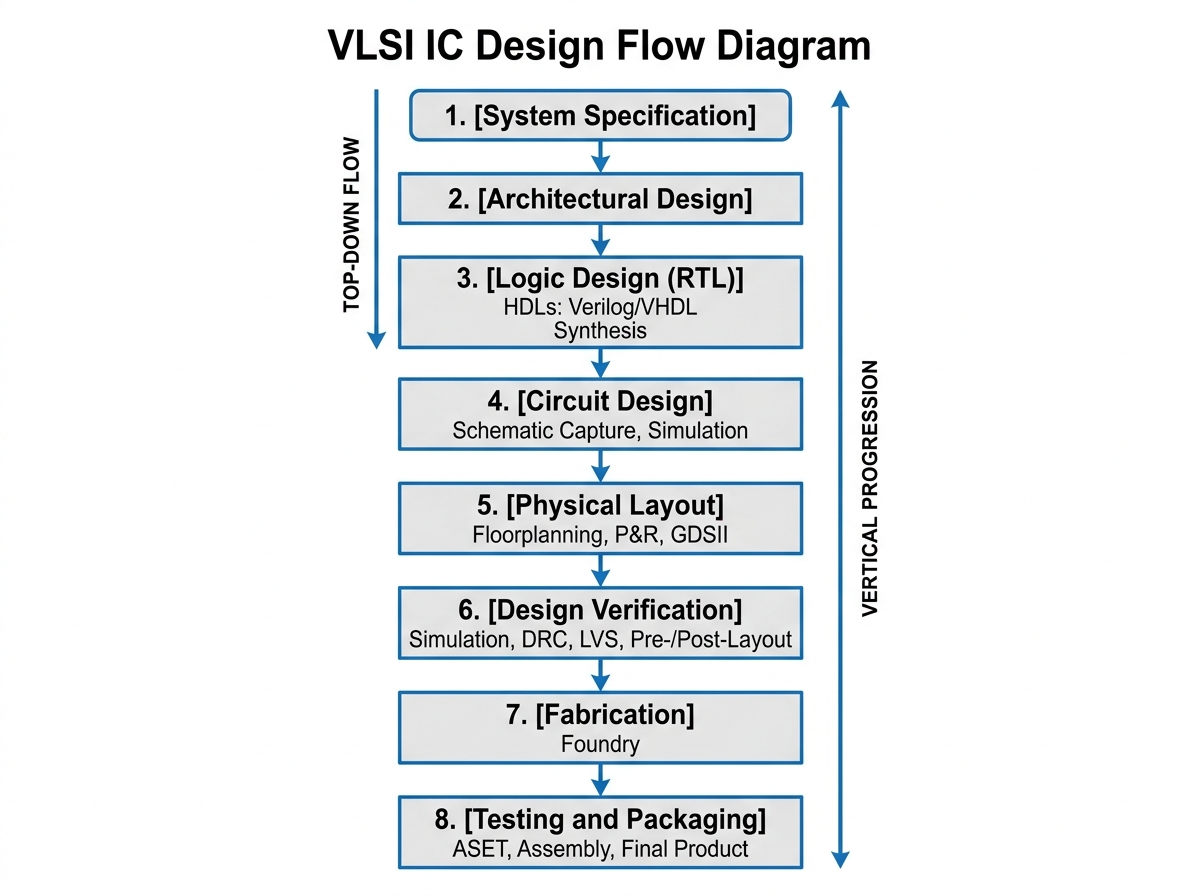
\includegraphics[width=0.75\textwidth]{vlsi_design_flow.jpg}
\caption{Standard VLSI IC design flow showing the hierarchical progression from system specification through architectural design, logic synthesis, circuit design, physical layout, design verification, fabrication, and testing.}
\label{fig:vlsi_flow}
\end{figure}

The VLSI design flow consists of the following major stages:

\noindent\textbf{1. System Specification:} This initial phase defines the overall functional requirements, performance targets (clock frequency, throughput), power budget, die area constraints, and target technology node for the integrated circuit.

\noindent\textbf{2. Architectural Design:} The system is partitioned into major functional blocks (processor cores, memory arrays, I/O interfaces, analog subsystems), and their interconnections are defined. Block-level timing and power budgets are allocated.

\noindent\textbf{3. Logic Design (RTL):} Each functional block is described using Hardware Description Languages (HDLs) such as Verilog or VHDL at the Register Transfer Level (RTL). Logic synthesis tools then map the RTL description to a technology-specific gate-level netlist using standard cell libraries.

\noindent\textbf{4. Circuit Design:} At this level, individual logic gates and custom circuits are designed at the transistor level, optimizing transistor sizing ($W/L$ ratios), logic style selection (CMOS, PTL, TGL, GDI), and supply voltage to meet performance, power, and area targets. This thesis operates primarily at this design level.

\noindent\textbf{5. Physical Layout:} The transistor-level circuit is translated into geometric mask patterns that define the physical locations and dimensions of transistors, interconnect wires, contacts, and vias on the silicon die.

\noindent\textbf{6. Design Verification:} The completed design is verified through Design Rule Checks (DRC), Layout vs. Schematic (LVS) comparisons, and post-layout parasitic extraction followed by timing and power simulations to ensure the physical design meets all specifications.

\noindent\textbf{7. Fabrication:} The verified mask set is sent to a semiconductor foundry (such as TSMC, Samsung, or GlobalFoundries) for photolithographic fabrication on silicon wafers.

\noindent\textbf{8. Testing and Packaging:} Fabricated dies are probed, tested for functional correctness and parametric compliance, then packaged into appropriate IC packages for deployment in electronic systems.

The circuit-level optimization explored in this thesis (Stage 4) directly impacts all subsequent stages, as a more efficient transistor-level design produces smaller layouts, lower power consumption, and improved system-level performance.

\section{Digital Comparators in Modern VLSI Architectures}

Among fundamental digital building blocks, the binary magnitude comparator is of central importance across computing architectures. A magnitude comparator is a combinational digital circuit that receives two binary words as inputs and evaluates their relative arithmetic values, asserting output flags to indicate whether the first input is greater than, equal to, or less than the second input [1]. Figure~\ref{fig:comparator_block} presents the functional block diagram of a 1-bit magnitude comparator.

\begin{figure}[H]
\centering
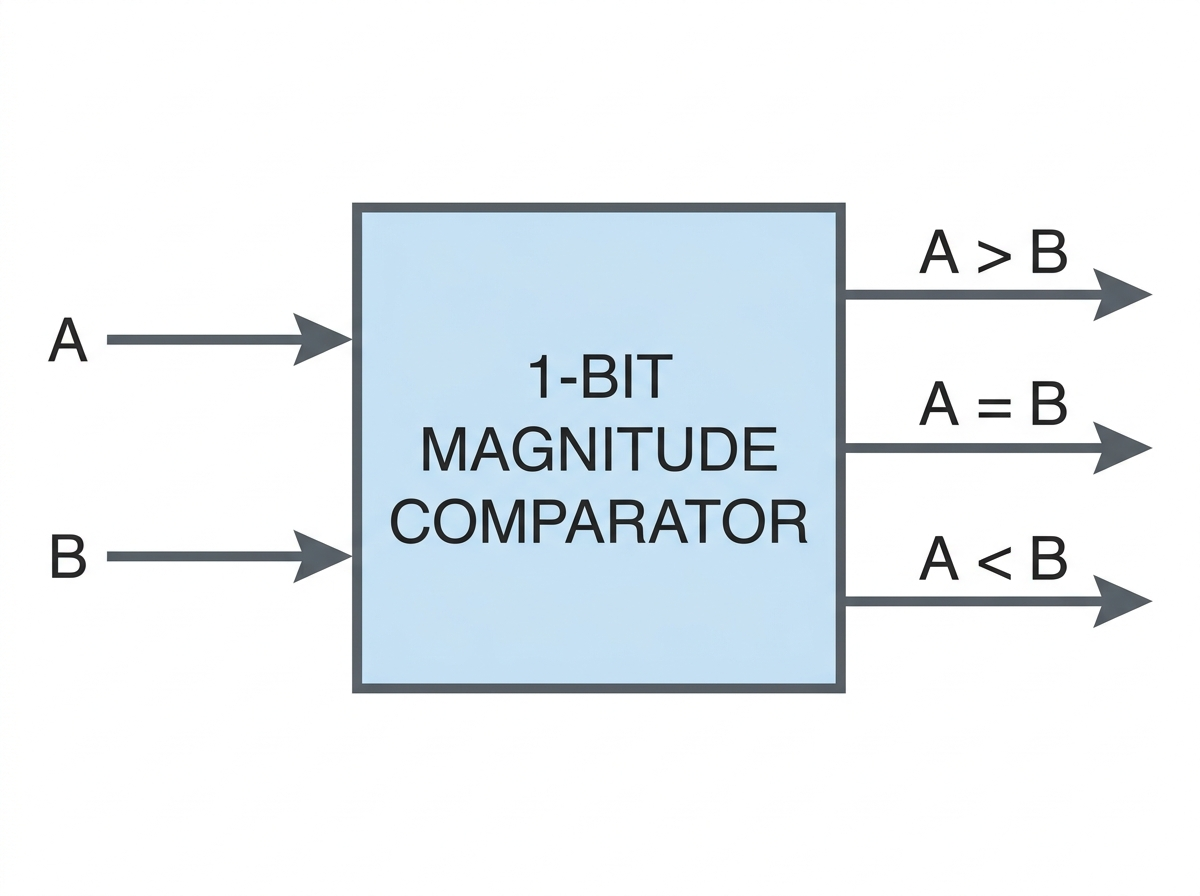
\includegraphics[width=0.6\textwidth]{comparator_block_diagram.jpg}
\caption{Functional block diagram of a 1-bit magnitude comparator with two single-bit inputs ($A$ and $B$) and three comparison outputs ($A>B$, $A=B$, $A<B$).}
\label{fig:comparator_block}
\end{figure}

At the most fundamental level, a 1-bit magnitude comparator processes two single-bit binary inputs, designated as $A$ and $B$, and generates three distinct output signals:
\begin{align}
\text{Greater-Than Output: } & A > B \\
\text{Equality Output: } & A = B \\
\text{Less-Than Output: } & A < B
\end{align}

Although a 1-bit comparator represents an elementary logical module, it forms the core building block for multi-bit ($n$-bit) comparators, tree comparators, priority encoders, and arithmetic sorting networks. In wide data-path architectures, single-bit comparator stages are cascaded in iterative or parallel-prefix arrangements to process word lengths of 8, 16, 32, and 64 bits [2].

Digital magnitude comparators perform indispensable computational roles across modern electronic systems:
\begin{itemize}
\item \textbf{Arithmetic Logic Units and Microprocessors:} Comparators execute conditional branch evaluation, loop termination checks, zero detection, sorting operations, relational operations, and data dependency checks in out-of-order execution pipelines [3].
\item \textbf{Flash Analog-to-Digital Converters (ADCs):} In ultra-high-speed Flash ADCs, arrays of digital comparators decode thermometer codes generated by analog preamplifiers into standard binary representations at gigahertz sampling rates. The power dissipation and latency of the comparator array directly dictate the overall energy efficiency and effective number of bits (ENOB) of the converter [1].
\item \textbf{Cache Memory and Content-Addressable Memory (CAM):} Comparators perform high-speed address tag-matching in Translation Lookaside Buffers (TLBs) and multi-level cache hierarchies, where comparison latency directly impacts CPU instruction throughput [4].
\item \textbf{Digital Signal Processing (DSP) and Image Processing:} Comparators are used extensively in median filtering, peak detection, Viterbi decoders, motion estimation engines, and neural network activation thresholding [2].
\item \textbf{Ultra-Low-Power Biomedical and IoT Devices:} In implantable pacemakers, neural recording interfaces, and environmental sensor nodes, comparators evaluate biosignals against safety thresholds to trigger duty-cycled wake-up sequences, preserving battery energy [3].
\item \textbf{Data Sorting and Search Engines:} In hardware-accelerated database engines and network packet classifiers, comparators form the basis of sorting networks (bitonic sorters, odd-even merge sorters) that process data at wire speed [6].
\end{itemize}

Given the widespread use of digital comparators, any architectural optimization that reduces transistor count, power consumption, or propagation delay in the elementary 1-bit comparator cell provides compounding improvements across the entire computational pipeline.

\section{Comparative Overview of Digital Logic Design Paradigms}

Over the history of VLSI design, various digital logic styles have been developed, each presenting distinct trade-offs among switching speed, power dissipation, silicon area, noise immunity, and design complexity:

\subsection{Static Complementary CMOS Logic (C-CMOS)}
Conventional static CMOS employs complementary pull-up (PMOS) and pull-down (NMOS) networks. For an $N$-input gate, static CMOS requires $2N$ transistors. While offering rail-to-rail voltage swing ($V_{OL}=0\text{V}$, $V_{OH}=V_{DD}$) and strong noise margins, static CMOS requires approximately 32 transistors for a 1-bit magnitude comparator, resulting in elevated parasitic load capacitance and higher dynamic switching power [1].

\subsection{Pass Transistor Logic (PTL)}
Pass Transistor Logic uses NMOS transistors as series pass elements to route input signals directly to the output. By eliminating separate pull-up networks, PTL reduces transistor count to 10 transistors for a 1-bit comparator. However, an NMOS transistor passing a logic high output produces a degraded voltage of $V_{DD} - V_{thn}$, where $V_{thn}$ is heightened by the body effect. This threshold drop degrades noise margins and leads to static current leakage in subsequent logic gates [2].

\subsection{Transmission Gate Logic (TGL)}
Transmission Gate Logic places an NMOS and a PMOS transistor in parallel to form a bidirectional switch controlled by complementary signals. TGL provides full rail-to-rail voltage transmission, eliminating the threshold drop of PTL. However, TGL requires complementary control signals for each switch, necessitating inverter stages and resulting in higher transistor count (16 to 24 transistors for a 1-bit comparator) and increased control-signal routing overhead [3].

\subsection{Gate Diffusion Input (GDI) Technique}
The Gate Diffusion Input (GDI) technique, introduced by Morgenshtein, Fish, and Wagner in 2002 [5], provides a compact alternative. A basic GDI cell consists of a single PMOS and NMOS transistor pair with three independently driven input terminals: common gate ($G$), PMOS diffusion ($P$), and NMOS diffusion ($N$). By configuring these three terminals, a single 2-transistor GDI cell can implement complex functions (2:1 MUX, AND, OR, XOR/XNOR) that require 6 to 12 transistors in conventional static CMOS [5]. This allows a complete 1-bit magnitude comparator to be implemented using only 10 transistors, achieving substantial reductions in switched capacitance, silicon area, and power dissipation [4].

\subsection{Summary Comparison of Logic Styles}

Table~\ref{tab:logic_styles_summary} summarizes the key characteristics of the four logic design paradigms discussed above, specifically in the context of implementing a 1-bit magnitude comparator.

\begin{table}[H]
\centering
\caption{Summary comparison of digital logic design styles for 1-bit magnitude comparator implementation.}
\label{tab:logic_styles_summary}
\vspace{0.2cm}
\begin{tabular}{|p{3.2cm}|c|c|c|c|}
\hline
\textbf{Characteristic} & \textbf{Static CMOS} & \textbf{PTL} & \textbf{TGL} & \textbf{GDI} \\
\hline
Transistor Count & 32 & 10 & 16--24 & 10 \\
\hline
Output Voltage Swing & Full rail & Degraded & Full rail & Near full \\
\hline
Noise Margin & Excellent & Poor & Good & Good \\
\hline
Dynamic Power & High & Low & Moderate & Very Low \\
\hline
Static Leakage & Moderate & High & Moderate & Low \\
\hline
Design Complexity & Moderate & Low & Moderate & Low \\
\hline
Area & Large & Small & Moderate & Small \\
\hline
\end{tabular}
\end{table}

\section{Motivation and Research Drivers}

The continuous growth of mobile computing, wearable technology, and Internet-of-Things (IoT) platforms demands digital circuits that operate under strict energy constraints. In these applications, battery longevity is the primary performance metric, and circuit blocks must operate with minimal power budgets [3].

Because digital comparators are among the most frequently executed primitives in arithmetic and signal-processing pipelines, optimizing their power consumption and silicon footprint directly benefits system-level energy efficiency. Conventional static CMOS comparators, while reliable, require 32 transistors and suffer from high parasitic capacitance. Alternative approaches such as PTL introduce voltage degradation, while TGL and hybrid techniques introduce structural complexity and higher device counts (16 to 24 transistors) [3, 4].

The Gate Diffusion Input (GDI) technique offers a compelling solution by enabling complex logic operations with minimal device count. A pure GDI-based comparator requires only 10 transistors, substantially reducing parasitic capacitances, active dynamic switching power, and static leakage currents. These advantages motivate the detailed design, modeling, and performance evaluation of a pure GDI 1-bit magnitude comparator presented in this thesis [1].

The specific motivating factors for this research include:
\begin{enumerate}
\item \textbf{Power Crisis in Modern VLSI:} The breakdown of Dennard scaling has made power consumption the primary design bottleneck in integrated circuit design.
\item \textbf{Growing IoT Market:} The projected deployment of over 75 billion IoT devices by 2030 demands ultra-low-power circuit primitives.
\item \textbf{Biomedical Applications:} Implantable medical devices require circuits operating in the picowatt to nanowatt power range for extended battery life.
\item \textbf{GDI Potential Underexplored:} Despite the proven advantages of GDI technique, comprehensive benchmarking studies of pure GDI comparators against multiple logic styles remain limited in the published literature.
\item \textbf{Academic Research Contribution:} This work contributes to the growing body of knowledge on low-power digital circuit design using alternative logic methodologies.
\end{enumerate}

\section{Problem Statement}

Digital magnitude comparators are fundamental combinational blocks in modern arithmetic engines and data converters. In deep-submicron VLSI technologies, these circuits must simultaneously deliver ultra-low power dissipation, short propagation delay, and compact silicon area.

Conventional static CMOS comparators require 32 transistors, leading to elevated power dissipation, substantial parasitic loading, and large layout area [1]. Pass Transistor Logic reduces device count but suffers from threshold voltage drops ($V_{DD} - V_{th}$) that compromise noise margins [2]. Transmission Gate Logic provides full rail-to-rail voltage swing but requires 16 to 24 transistors and dual-rail control routing [3]. Recent hybrid topologies combine multiple logic styles but typically require 24 or more transistors and introduce complex interconnect interfaces [4].

Therefore, there is a clear need for an optimized 1-bit magnitude comparator that achieves minimal transistor count, eliminates unnecessary driving stages, minimizes average power dissipation, and delivers competitive propagation delay without compromising functional correctness.

This research addresses these challenges by developing a 10-transistor 1-bit magnitude comparator implemented entirely using the Gate Diffusion Input (GDI) technique, and performing comprehensive performance benchmarking against conventional CMOS, PTL, and TGL topologies at the 180nm CMOS technology node under consistent operating conditions.

\section{Research Objectives}

The primary objectives of this thesis are:

\begin{enumerate}
\item \textbf{Theoretical Investigation:} To conduct a rigorous mathematical and structural analysis of 1-bit digital magnitude comparator architectures, establishing Boolean expressions, truth tables, and switching characteristics for all three comparison outputs ($A>B$, $A=B$, and $A<B$).
\item \textbf{GDI Circuit Synthesis:} To synthesize an optimized 1-bit magnitude comparator circuit utilizing the Gate Diffusion Input (GDI) methodology, realizing all three comparison functions using a minimal footprint of only 10 transistors.
\item \textbf{Benchmark Circuit Modeling:} To design, model, and simulate reference comparator topologies—including a 32-transistor conventional static CMOS comparator, a 10-transistor pass transistor logic (PTL) comparator, and a 16-transistor transmission gate logic (TGL) comparator—under identical electrical constraints.
\item \textbf{Simulation and Functional Verification:} To perform transient SPICE simulations in LTSpice using the Berkeley Predictive Technology Model (PTM) at the 180nm technology node with a 1.8V power supply, confirming functional correctness across all four input state combinations.
\item \textbf{Performance Characterization:} To extract and quantify key performance metrics across all evaluated topologies, including rise time ($t_r$), fall time ($t_f$), propagation delay ($t_{pd}$), average power dissipation ($P_{avg}$), and Power-Delay Product (PDP).
\item \textbf{Comparative Literature Benchmarking:} To systematically compare the obtained simulation metrics against state-of-the-art comparator designs published in IEEE literature ([1]--[4]).
\item \textbf{Technology Node Scaling Evaluation:} To evaluate the scalability of the comparator architectures across advanced nanometer nodes (180nm, 90nm, and 45nm PTM).
\item \textbf{Engineering Impact Assessment:} To analyze the societal, environmental, sustainability, and complex engineering problem-solving attributes (P1--P7) and activities (A1--A5) associated with low-power VLSI design.
\end{enumerate}

\section{Research Methodology}

The investigation follows a structured four-phase engineering research methodology:

\noindent\textbf{Phase 1: Analytical Formulation and Literature Survey}\\
An extensive review of digital comparator designs, low-power logic styles (CMOS, PTL, TGL, GDI, and hybrid styles), and MOSFET leakage physics was performed. Benchmark papers [1]--[4] were analyzed in detail to establish performance baselines.

\noindent\textbf{Phase 2: Mathematical Derivation and Circuit Topology Design}\\
Boolean functions for $A>B$, $A=B$, and $A<B$ were derived and mapped to optimal GDI cell configurations. Sizing ratios ($W/L$) for all NMOS and PMOS transistors were calculated to balance high-to-low and low-to-high switching transitions. Benchmark circuits (Static CMOS, PTL, TGL) were designed using consistent device models.

\noindent\textbf{Phase 3: LTSpice Modeling and Transient Simulation}\\
All comparator circuits were implemented in LTSpice using BSIM3v3 Predictive Technology Model (PTM) 180nm device parameters. Transient pulse trains were configured to test all input transitions ($00 \rightarrow 01 \rightarrow 10 \rightarrow 11$). High-precision transient (.tran) analyses were executed over a 100ns window.

\noindent\textbf{Phase 4: Parameter Extraction, Analysis, and Validation}\\
Waveform post-processing was conducted to compute rise times, fall times, propagation delays ($t_{pHL}$, $t_{pLH}$, and average $t_{pd}$), continuous integral power dissipation, and Power-Delay Product (PDP). Multi-node technology scaling simulations (180nm, 90nm, 45nm) and comparative literature analyses were completed.

\section{Scope and Delimitations of the Study}

The boundaries of this study are defined as follows:
\begin{itemize}
\item The investigation focuses on 1-bit magnitude comparator architectures evaluating three binary outputs: $A>B$, $A=B$, and $A<B$.
\item Transistor-level circuit design and SPICE-level transient simulations are conducted using LTSpice with BSIM3v3 Predictive Technology Model (PTM) parameter decks at the 180nm technology node ($V_{DD} = 1.8\text{V}$), with scaling evaluations at 90nm and 45nm.
\item Circuit evaluations are based on schematic-level simulations with lumped parasitic models. Physical silicon mask fabrication and physical cleanroom testing are excluded due to resource constraints.
\item The study does not include Monte Carlo statistical process variation analysis or full PVT corner characterization, which are recommended as future work.
\item Fan-out loading effects and interconnect RC delay modeling are not included in the current evaluation, as the focus is on intrinsic cell-level performance.
\end{itemize}

\section{Thesis Organization}

The remainder of this thesis is structured as follows:

\noindent\textbf{Chapter 2: Literature Review}\\
Presents the theoretical foundation of binary magnitude comparators, MOSFET power dissipation mechanisms, and operational principles of static CMOS, PTL, TGL, and GDI logic. A detailed review of key published works ([1]--[4]), a comparative summary table, and a research gap analysis are provided.

\noindent\textbf{Chapter 3: Methodology}\\
Details the system specifications, mathematical derivations, truth tables, logic mappings, transistor-level schematics, device sizing strategies, and simulation testbench setup in LTSpice.

\noindent\textbf{Chapter 4: Results and Discussion}\\
Presents simulation waveforms, functional verification, timing analyses, power dissipation measurements, comparative performance tables, technology scaling investigations (180nm, 90nm, 45nm), literature comparisons, and assessments of societal, health, environmental, and sustainability impacts.

\noindent\textbf{Chapter 5: Conclusions and Future Work}\\
Summarizes the major findings, highlights technical contributions, discusses study limitations, and outlines recommendations for future research extensions.

\noindent\textbf{References and Appendices}\\
Includes IEEE-formatted bibliographic citations ([1]--[12]) followed by Appendix A (Simulation Configuration), Appendix B (Complex Engineering Problem Attributes P1--P7), Appendix C (Complex Engineering Activities A1--A5), and Appendix D (Mathematical Models of Leakage and GDI Conduction).


% ############################################################################
% CHAPTER 2: LITERATURE REVIEW
% ############################################################################
\chapter{LITERATURE REVIEW}

\section{Introduction}

This chapter presents a detailed review of the theoretical concepts, semiconductor physics, circuit topologies, and published literature relevant to digital magnitude comparator design in low-power VLSI systems. It begins with the mathematical foundations of binary magnitude comparison and an examination of power dissipation mechanisms in deep-submicron MOSFETs. Next, it analyzes conventional static CMOS logic and alternative logic styles, including Pass Transistor Logic (PTL), Transmission Gate Logic (TGL), and Gate Diffusion Input (GDI). The chapter then presents a detailed critical analysis of four benchmark papers ([1]--[4]), followed by a comparative summary table and a research gap analysis that justifies the proposed GDI comparator architecture.

\section{Fundamentals of Binary Magnitude Comparators}

A binary magnitude comparator is a fundamental combinational digital block that compares two binary words and determines their relative numerical relationship. For two single-bit inputs $A$ and $B$, the comparator evaluates three arithmetic conditions:
\begin{enumerate}
\item \textbf{Greater-Than Condition ($A>B$):} The output evaluates to logic high ($1$) if and only if $A=1$ and $B=0$.
\item \textbf{Equality Condition ($A=B$):} The output evaluates to logic high ($1$) if and only if both bits are identical, i.e., $A=B=0$ or $A=B=1$.
\item \textbf{Less-Than Condition ($A<B$):} The output evaluates to logic high ($1$) if and only if $A=0$ and $B=1$.
\end{enumerate}

The functional behavior is completely defined by the truth table shown in Table~\ref{tab:lit_truthtable}.

\begin{table}[H]
\centering
\caption{Complete truth table for a 1-bit binary magnitude comparator.}
\label{tab:lit_truthtable}
\vspace{0.2cm}
\begin{tabular}{|c|c|c|c|c|}
\hline
\textbf{Input A} & \textbf{Input B} & \textbf{Output ($A>B$)} & \textbf{Output ($A=B$)} & \textbf{Output ($A<B$)} \\
\hline
0 & 0 & 0 & 1 & 0 \\
\hline
0 & 1 & 0 & 0 & 1 \\
\hline
1 & 0 & 1 & 0 & 0 \\
\hline
1 & 1 & 0 & 1 & 0 \\
\hline
\end{tabular}
\end{table}

Applying canonical sum-of-products (SOP) formulation to Table~\ref{tab:lit_truthtable} yields the governing Boolean equations:

\begin{equation}
(A > B) = A \cdot \overline{B}
\label{eq:lit_agb}
\end{equation}

\begin{equation}
(A = B) = \overline{A}\,\overline{B} + A B = \overline{A \oplus B} = A \odot B
\label{eq:lit_aeb}
\end{equation}

\begin{equation}
(A < B) = \overline{A} \cdot B
\label{eq:lit_alb}
\end{equation}

\subsection{Karnaugh Map Minimization}

The Boolean expressions can also be derived through Karnaugh map (K-map) minimization, which provides a graphical method for simplifying Boolean functions. For a 1-bit comparator with two input variables $A$ and $B$, the K-maps are straightforward:

\noindent\textbf{K-map for $A > B$:}

\begin{center}
\begin{tabular}{c|c|c|}
\multicolumn{1}{c}{} & \multicolumn{1}{c}{$B=0$} & \multicolumn{1}{c}{$B=1$} \\
\cline{2-3}
$A=0$ & 0 & 0 \\
\cline{2-3}
$A=1$ & 1 & 0 \\
\cline{2-3}
\end{tabular}
\end{center}

\noindent The single minterm $m_2$ ($A=1, B=0$) yields: $(A > B) = A \cdot \overline{B}$.

\noindent\textbf{K-map for $A = B$:}

\begin{center}
\begin{tabular}{c|c|c|}
\multicolumn{1}{c}{} & \multicolumn{1}{c}{$B=0$} & \multicolumn{1}{c}{$B=1$} \\
\cline{2-3}
$A=0$ & 1 & 0 \\
\cline{2-3}
$A=1$ & 0 & 1 \\
\cline{2-3}
\end{tabular}
\end{center}

\noindent The two diagonal minterms $m_0$ and $m_3$ cannot be grouped in a standard K-map adjacency, yielding: $(A = B) = \overline{A}\,\overline{B} + AB = A \odot B$ (XNOR operation).

\noindent\textbf{K-map for $A < B$:}

\begin{center}
\begin{tabular}{c|c|c|}
\multicolumn{1}{c}{} & \multicolumn{1}{c}{$B=0$} & \multicolumn{1}{c}{$B=1$} \\
\cline{2-3}
$A=0$ & 0 & 1 \\
\cline{2-3}
$A=1$ & 0 & 0 \\
\cline{2-3}
\end{tabular}
\end{center}

\noindent The single minterm $m_1$ ($A=0, B=1$) yields: $(A < B) = \overline{A} \cdot B$.

\subsection{Extension to Multi-Bit Comparators}

In multi-bit digital systems comparing two $n$-bit binary words $A = (A_{n-1} A_{n-2} \dots A_0)$ and $B = (B_{n-1} B_{n-2} \dots B_0)$, the comparison starts from the most significant bit (MSB) position $n-1$ and ripples down toward the least significant bit (LSB). The overall equality condition requires that every individual bit pair evaluates to equivalence:
\begin{equation}
(A = B)_n = \prod_{k=0}^{n-1} (A_k \odot B_k)
\end{equation}
The greater-than condition for an $n$-bit word is evaluated hierarchically as:
\begin{equation}
(A > B)_n = (A_{n-1} \overline{B_{n-1}}) + (A_{n-1} \odot B_{n-1})(A_{n-2} \overline{B_{n-2}}) + \dots + \left[\prod_{k=1}^{n-1} (A_k \odot B_k)\right](A_0 \overline{B_0})
\end{equation}
Similarly, the less-than condition is expressed as:
\begin{equation}
(A < B)_n = (\overline{A_{n-1}} B_{n-1}) + (A_{n-1} \odot B_{n-1})(\overline{A_{n-2}} B_{n-2}) + \dots + \left[\prod_{k=1}^{n-1} (A_k \odot B_k)\right](\overline{A_0} B_0)
\end{equation}

Because multi-bit comparators rely directly on the repeated replication of the elementary 1-bit comparator cell, optimizing the power, delay, and transistor count of the 1-bit cell yields compounded benefits across wide data paths. For instance, a 32-bit comparator constructed from optimized 1-bit GDI cells would require $32 \times 10 = 320$ transistors, compared to $32 \times 32 = 1024$ transistors using conventional static CMOS logic—a saving of 704 transistors per comparator instance.

\section{MOSFET Power Dissipation Mechanisms}

Power dissipation in digital CMOS VLSI circuits comprises three primary components: dynamic switching power ($P_{dyn}$), short-circuit power ($P_{sc}$), and static leakage power ($P_{stat}$) [6]:

\begin{equation}
P_{total} = P_{dyn} + P_{sc} + P_{stat}
\label{eq:ptotal}
\end{equation}

\subsection{Dynamic Switching Power ($P_{dyn}$)}
Dynamic switching power occurs during logic state transitions when parasitic load capacitances are charged from $V_{DD}$ and discharged to ground. Over a clock period $T = 1/f$, the dynamic power is given by:
\begin{equation}
P_{dyn} = \alpha_{0 \rightarrow 1} \cdot C_{load} \cdot V_{DD}^2 \cdot f
\label{eq:pdyn}
\end{equation}
where $\alpha_{0 \rightarrow 1}$ represents the switching activity factor (the probability that a power-consuming transition occurs per clock cycle), $C_{load}$ is the total effective output load capacitance (including transistor gate, drain diffusion, and interconnect capacitances), $V_{DD}$ is the supply voltage, and $f$ is the operational frequency. Reducing the total number of transistors in a logic network directly decreases $C_{load}$, yielding quadratic power savings [7].

Dynamic power is the dominant component of total power dissipation in circuits operating at high frequencies and at technology nodes above 90nm. The quadratic dependence on $V_{DD}$ makes supply voltage reduction the most effective strategy for dynamic power minimization; however, reducing $V_{DD}$ also increases propagation delay and reduces noise margins.

\subsection{Short-Circuit Power ($P_{sc}$)}
During an input transition, when the input voltage crosses the region between $V_{thn}$ and $V_{DD} - |V_{thp}|$, both the NMOS pull-down and PMOS pull-up networks conduct simultaneously for a brief duration $t_{sc}$. This creates a direct current path between $V_{DD}$ and ground:
\begin{equation}
P_{sc} = I_{peak} \cdot t_{sc} \cdot V_{DD} \cdot f = \frac{\beta}{12} (V_{DD} - 2V_{th})^3 \frac{t_r + t_f}{T}
\end{equation}
Short-circuit power typically accounts for 10\% to 20\% of total dynamic power in well-designed static CMOS circuits. By minimizing intermediate switching stages, alternative logic styles can reduce short-circuit dissipation [8].

\subsection{Static Leakage Power ($P_{stat}$)}
Static power dissipation occurs when transistors are in the steady-state (quiescent) condition:
\begin{equation}
P_{stat} = I_{leakage} \cdot V_{DD}
\end{equation}
In deep-submicron regime (180nm and below), $I_{leakage}$ is governed by several physical mechanisms [12]:
\begin{enumerate}
\item \textbf{Subthreshold Leakage Current ($I_{sub}$):} Current flowing between the drain and source when the gate-to-source voltage $V_{gs}$ is below the threshold voltage $V_{th}$:
\begin{equation}
I_{sub} = \mu_0 C_{ox} \frac{W}{L} (m-1) v_T^2 \exp\left(\frac{V_{gs} - V_{th}}{m v_T}\right) \left[1 - \exp\left(-\frac{V_{ds}}{v_T}\right)\right]
\label{eq:isub}
\end{equation}
where $\mu_0$ is carrier mobility, $C_{ox}$ is gate oxide capacitance per unit area, $W/L$ is the transistor aspect ratio, $v_T = k_B T / q$ is thermal voltage ($\approx 26\text{mV}$ at $300\text{K}$), and $m$ is the subthreshold swing coefficient.
\item \textbf{Drain-Induced Barrier Lowering (DIBL):} In short-channel MOSFETs, high drain bias lowers the channel potential barrier, shifting the threshold voltage downward:
\begin{equation}
\Delta V_{th} = -\eta V_{ds}
\end{equation}
where $\eta$ is the DIBL coefficient. This barrier reduction exponentially increases subthreshold leakage current.
\item \textbf{Gate-Induced Drain Leakage (GIDL):} High electric fields in the drain-gate overlap region induce band-to-band tunneling, generating leakage current from drain to substrate.
\item \textbf{Gate-Oxide Direct Tunneling ($I_{gate}$):} Thin dielectric oxide layers allow direct quantum-mechanical electron tunneling from the gate to the channel and substrate.
\end{enumerate}

Table~\ref{tab:leakage_summary} summarizes the relative significance of each leakage mechanism across different technology nodes.

\begin{table}[H]
\centering
\caption{Relative significance of leakage mechanisms across CMOS technology nodes.}
\label{tab:leakage_summary}
\vspace{0.2cm}
\begin{tabular}{|l|c|c|c|}
\hline
\textbf{Leakage Mechanism} & \textbf{180nm} & \textbf{90nm} & \textbf{45nm} \\
\hline
Subthreshold ($I_{sub}$) & Moderate & High & Very High \\
\hline
DIBL & Low & Moderate & High \\
\hline
GIDL & Low & Low & Moderate \\
\hline
Gate Tunneling ($I_{gate}$) & Negligible & Low & Moderate \\
\hline
\end{tabular}
\end{table}

\section{Analysis of Digital Logic Styles}

\subsection{Conventional Static CMOS Logic}
Conventional static CMOS logic constructs logic functions using complementary PMOS pull-up and NMOS pull-down networks. Figure~\ref{fig:static_comp} illustrates the static CMOS 1-bit comparator circuit.

\noindent\textbf{Advantages:}
\begin{itemize}
\item Robust noise margins ($SNM \approx V_{DD}/2$).
\item Full rail-to-rail output swing without threshold attenuation.
\item Well-established automated synthesis and standard-cell library support [7].
\item Zero static power dissipation in ideal conditions (no DC path between $V_{DD}$ and ground in steady state).
\item High reliability and process tolerance.
\end{itemize}

\noindent\textbf{Disadvantages:}
\begin{itemize}
\item High device count ($2N$ transistors for $N$ inputs).
\item High total switched load capacitance ($C_{load}$).
\item Significant silicon area footprint and multi-path static leakage [8].
\item Large input capacitance due to both NMOS and PMOS gate loads.
\end{itemize}

\subsection{Pass Transistor Logic (PTL)}
Pass Transistor Logic uses NMOS transistors as series switching elements to route inputs directly to output nodes. Figure~\ref{fig:pass_comp} shows the 10-transistor PTL comparator schematic.

\noindent\textbf{Advantages:}
\begin{itemize}
\item Substantially reduced transistor count (10 transistors for 1-bit comparator).
\item Lower input gate capacitance and reduced dynamic power [6].
\item Compact layout area due to fewer transistors.
\item Faster switching for certain logic functions due to reduced parasitic loading.
\end{itemize}

\noindent\textbf{Disadvantages:}
\begin{itemize}
\item Output voltage degradation ($V_{out} \le V_{DD} - V_{thn}$), resulting in reduced noise margins.
\item Elevated body effect due to non-zero source-to-substrate voltage ($V_{sb} > 0$), which further increases $V_{thn}$ according to Equation~\ref{eq:bodyeffect}.
\item Increased subthreshold leakage in downstream logic driven by degraded high levels [12].
\item Requires level-restoring circuits for cascaded stages, which adds transistor count.
\item Signal integrity degrades in long pass-transistor chains.
\end{itemize}

\subsection{Transmission Gate Logic (TGL)}
Transmission Gate Logic places an NMOS and a PMOS transistor in parallel to create a bidirectional transmission switch controlled by complementary signals ($C$ and $\overline{C}$). Figure~\ref{fig:tg_comp} shows the 16-transistor TGL comparator schematic.

\noindent\textbf{Advantages:}
\begin{itemize}
\item Full rail-to-rail voltage transfer: NMOS passes logic low ($0\text{V}$) without degradation, while PMOS passes logic high ($V_{DD}$) without attenuation.
\item Lower equivalent on-resistance across the full voltage range [7].
\item No threshold voltage drop in output signals.
\item Good noise margins approaching static CMOS levels.
\end{itemize}

\noindent\textbf{Disadvantages:}
\begin{itemize}
\item Requires complementary control signals, necessitating additional inverter stages.
\item Higher transistor count than PTL (16 to 24 transistors).
\item Increased interconnect routing complexity for dual-rail control signals [3].
\item Higher dynamic power than PTL due to increased switching capacitance from complementary control nets.
\end{itemize}

\subsection{Gate Diffusion Input (GDI) Technique}

Introduced by Morgenshtein et al. in 2002 [5], the GDI technique employs a twin-transistor cell (one PMOS, one NMOS) with three independent terminals:
\begin{itemize}
\item $G$: Common gate input to both PMOS and NMOS.
\item $P$: Source/drain terminal of the PMOS transistor.
\item $N$: Source/drain terminal of the NMOS transistor.
\item $Out$: Common drain output node.
\end{itemize}

Figure~\ref{fig:gdi_cell} illustrates the basic GDI cell structure showing both the transistor-level schematic and the simplified block symbol.

\begin{figure}[H]
\centering
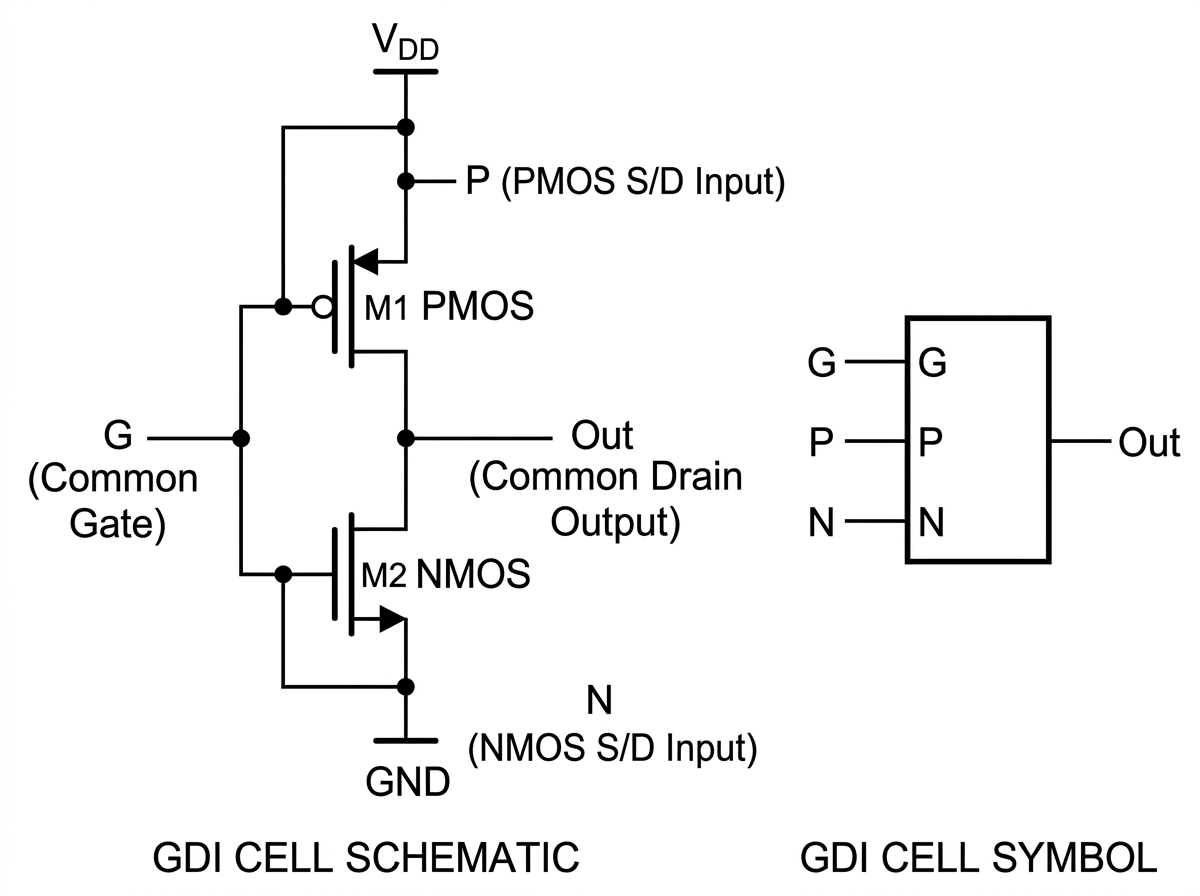
\includegraphics[width=0.75\textwidth]{gdi_cell_structure.jpg}
\caption{Basic Gate Diffusion Input (GDI) cell: (left) transistor-level schematic showing PMOS and NMOS with three independent input terminals $G$, $P$, $N$, and common drain output; (right) simplified GDI cell symbol.}
\label{fig:gdi_cell}
\end{figure}

By connecting the $P$, $N$, and $G$ terminals to appropriate logic signals, supply voltages, or ground, a single GDI cell can implement six distinct logical operations, as detailed in Table~\ref{tab:lit_gdifunc}.

\begin{table}[H]
\centering
\caption{Operational configurations and Boolean logic functions of a basic 2T GDI cell.}
\label{tab:lit_gdifunc}
\vspace{0.2cm}
\begin{tabular}{|c|c|c|c|c|c|}
\hline
\textbf{N Input} & \textbf{P Input} & \textbf{G Input} & \textbf{Output Function} & \textbf{Logic Operation} & \textbf{CMOS Transistors} \\
\hline
$0$ (GND) & $B$ & $A$ & $\overline{A} \cdot B$ & Function F1 (AND) & 6 \\
\hline
$B$ & $1$ ($V_{DD}$) & $A$ & $\overline{A} + B$ & Function F2 (OR) & 6 \\
\hline
$1$ ($V_{DD}$) & $B$ & $A$ & $A + B$ & OR Gate & 6 \\
\hline
$B$ & $0$ (GND) & $A$ & $A \cdot B$ & AND Gate & 6 \\
\hline
$C$ & $B$ & $A$ & $\overline{A} B + A C$ & 2:1 MUX & 12 \\
\hline
$0$ (GND) & $1$ ($V_{DD}$) & $A$ & $\overline{A}$ & Inverter (NOT) & 2 \\
\hline
\end{tabular}
\end{table}

\noindent\textbf{Advantages of the GDI Technique:}
\begin{itemize}
\item \textbf{Dramatic Transistor Count Reduction:} Complex operations such as 2:1 MUX and AND functions are realized using only 2 transistors rather than 6 to 12 in CMOS.
\item \textbf{Ultra-Low Power Dissipation:} Fewer transistors directly translate into reduced input gate capacitance, minimized internal node charging/discharging, and lowered dynamic power.
\item \textbf{Compact Die Area:} GDI layouts achieve significant area savings over equivalent static CMOS designs [5].
\item \textbf{Design Simplicity:} A uniform 2-transistor cell structure simplifies the design process and enables systematic logic mapping.
\item \textbf{Reduced Interconnect Complexity:} Fewer transistors lead to fewer routing channels and reduced parasitic interconnect capacitance.
\end{itemize}

\noindent\textbf{Design Considerations in GDI Circuits:}
In standard bulk CMOS processes with common $N$-well and $P$-substrate connections, the sources of PMOS and NMOS transistors in GDI cells are not always tied to $V_{DD}$ and GND. Consequently, varying source-to-substrate voltages ($V_{sb}$) can induce body effect shifts, slightly increasing $V_{th}$ for certain transition paths. In 180nm CMOS technology, this threshold shift is modest and does not prevent robust digital operation, as confirmed by our simulation results [5].

Additionally, GDI circuits may exhibit slightly degraded output voltage swing compared to full static CMOS in some configurations. However, the voltage degradation is typically less severe than in PTL circuits, and the output levels remain within acceptable logic margins for downstream gate driving. In twin-well or Silicon-on-Insulator (SOI) processes, where each transistor can have its body terminal independently connected, the body effect limitation is entirely eliminated, making GDI an even more attractive design choice.

\section{CMOS Technology Scaling Roadmap}

The International Technology Roadmap for Semiconductors (ITRS), now succeeded by the International Roadmap for Devices and Systems (IRDS), has historically guided the semiconductor industry's scaling trajectory. Table~\ref{tab:tech_roadmap} presents key parameters across technology nodes relevant to this study.

\begin{table}[H]
\centering
\caption{Key CMOS technology parameters across scaling nodes (ITRS/PTM data).}
\label{tab:tech_roadmap}
\vspace{0.2cm}
\begin{tabular}{|l|c|c|c|}
\hline
\textbf{Parameter} & \textbf{180nm} & \textbf{90nm} & \textbf{45nm} \\
\hline
Gate length ($L_{gate}$) & 180 nm & 90 nm & 45 nm \\
\hline
Supply voltage ($V_{DD}$) & 1.8 V & 1.2 V & 1.0 V \\
\hline
Gate oxide thickness ($t_{ox}$) & 4.0 nm & 2.2 nm & 1.4 nm \\
\hline
NMOS $V_{th0}$ (nominal) & $\sim$0.40 V & $\sim$0.30 V & $\sim$0.22 V \\
\hline
PMOS $|V_{th0}|$ (nominal) & $\sim$0.42 V & $\sim$0.32 V & $\sim$0.24 V \\
\hline
Subthreshold swing & $\sim$80 mV/dec & $\sim$85 mV/dec & $\sim$90 mV/dec \\
\hline
Leakage current density & Low & Moderate & High \\
\hline
\end{tabular}
\end{table}

As technology nodes scale from 180nm toward 45nm and beyond, the following trends significantly impact digital circuit design:
\begin{enumerate}
\item \textbf{Supply Voltage Reduction:} Lower $V_{DD}$ reduces dynamic power quadratically but also decreases noise margins and gate overdrive.
\item \textbf{Increased Leakage:} Thinner gate oxides and lower threshold voltages dramatically increase static leakage currents.
\item \textbf{Short-Channel Effects:} DIBL, velocity saturation, and hot-carrier effects become increasingly prominent at smaller nodes.
\item \textbf{Process Variability:} Random dopant fluctuation and line-edge roughness cause larger parametric variations at advanced nodes.
\end{enumerate}

\section{Detailed Review of Key Prior Works}

To establish the context of this study, four relevant benchmark research papers on digital comparator design were analyzed in detail.

\subsection{Work 1: Kumar and Kumar (2017) -- CMOS Stacking Technique}
\textbf{Citation:} A. Kumar and M. Kumar, ``Improved Design of CMOS 1-Bit Comparator with Stacking Technique,'' \textit{International Journal of Current Engineering and Technology}, Vol. 7, no. 3, pp. 1044--1047, 2017 [1].

\noindent\textbf{Summary:} This paper investigates a 1-bit CMOS comparator utilizing the transistor stacking technique to suppress active leakage currents. In this approach, each original transistor of width $W$ is split into two series-connected transistors of width $W/2$. When both series devices turn off, the intermediate node potential rises slightly above ground, inducing a reverse body-to-source bias ($V_{bs} < 0$) and a negative gate-to-source bias ($V_{gs} < 0$). This self-reverse bias effect exponentially curtails subthreshold leakage current according to Equation~\ref{eq:isub}.

\noindent\textbf{Key Findings and Metrics:}
\begin{itemize}
\item Technology node: TSMC 180nm CMOS with supply voltage varied from 1.0V to 2.8V.
\item Reported propagation delay: $49.38\text{ ns}$ at $V_{DD} = 1.8\text{V}$.
\item Reported power dissipation: $174.352\text{ pW}$.
\item Power-Delay Product: $0.0086\text{ fJ}$ ($8.6\times 10^{-18}\text{ J}$).
\item \textbf{Limitations:} Transistor count increases significantly because every single transistor is duplicated into a stacked series pair (requiring 45+ transistors), substantially increasing layout area and routing complexity [1].
\end{itemize}

\noindent\textbf{Critical Analysis:} While the stacking technique effectively reduces subthreshold leakage, the dramatically increased propagation delay (49.38 ns) makes this design unsuitable for high-speed applications. The large transistor count also negates much of the leakage power savings due to increased parasitic capacitance. Furthermore, the stacking technique introduces a performance-area trade-off that may not be favorable in area-constrained designs.

\subsection{Work 2: Tailor, Sharma, and Kumar (2019) -- MTCMOS and Forced Stacking}
\textbf{Citation:} D. Tailor, T. Sharma, and M. Kumar, ``Design of CMOS Based 1-bit Comparator with MTCMOS and Forced Stack Technique in 180$\mu$m Technology,'' in \textit{Proc. 2019 IEEE International Conference on Signal Processing and Communication (ICSC)}, NOIDA, India, pp. 330--334, 2019 [2].

\noindent\textbf{Summary:} Tailor et al. proposed a 1-bit comparator combining Multi-Threshold CMOS (MTCMOS) with forced stacking. The MTCMOS scheme inserts high-$V_{th}$ sleep transistors in series with the power rails to choke standby leakage paths, while low-$V_{th}$ devices execute high-speed logical transitions during active operation. Forced stacking was simultaneously applied to the internal logic network to suppress runtime active leakage.

\noindent\textbf{Key Findings and Metrics:}
\begin{itemize}
\item Technology node: 180nm SPICE simulation at $V_{DD} = 1.8\text{V}$.
\item Reported propagation delay: $330.61\text{ ps}$.
\item Reported power dissipation: $48.12\text{ pW}$.
\item Power-Delay Product: $0.0000159\text{ fJ}$ ($1.59\times 10^{-20}\text{ J}$).
\item \textbf{Limitations:} The dual-threshold fabrication process requires additional mask steps, increasing manufacturing cost. The design also requires sleep-signal generation circuitry and encounters wake-up latency overhead when transitioning between standby and active modes [2].
\end{itemize}

\noindent\textbf{Critical Analysis:} The MTCMOS approach achieves excellent standby leakage reduction but introduces significant complexity. The requirement for dual-$V_{th}$ device fabrication increases manufacturing cost and limits the technique to foundries offering multi-threshold process options. The wake-up latency from sleep mode can degrade system responsiveness in real-time applications. Additionally, the sleep transistor sizing must be carefully optimized to avoid excessive voltage drops during active operation, which can reduce effective noise margins.

\subsection{Work 3: Lubaba, Islam, Faisal, and Hasan (2020) -- Hybrid PTL-TG-CMOS Comparator}
\textbf{Citation:} S. Lubaba, M. S. Islam, K. M. Faisal, and M. Hasan, ``Design of a Two-Bit Magnitude Comparator Based on Pass Transistor, Transmission Gate and Conventional Static CMOS Logic,'' in \textit{Proc. 2020 IEEE Region 10 Symposium (TENSYMP)}, Dhaka, Bangladesh, pp. 1114--1117, 2020 [3].

\noindent\textbf{Summary:} Lubaba et al. presented a hybrid design methodology for a 2-bit magnitude comparator implemented in 90nm CMOS technology. The architecture selectively assigns logic styles to different functional stages: Pass Transistor Logic is used for input product terms, Transmission Gates implement multiplexing and XOR functions, and conventional CMOS inverters restore signal levels at the output stages.

\noindent\textbf{Key Findings and Metrics:}
\begin{itemize}
\item Technology node: Cadence Virtuoso 90nm node with $V_{DD} = 1.0\text{V}$.
\item Reported propagation delay: $0.192\text{ ns}$ ($192\text{ ps}$).
\item Reported power dissipation: $7.792\text{ }\mu\text{W}$.
\item Power-Delay Product: $1.496\text{ fJ}$.
\item \textbf{Limitations:} The design utilizes a large number of transistors due to the 2-bit wordlength and hybrid driving stages, resulting in elevated microwatt-level power consumption that is less suitable for ultra-low-power biomedical or energy-harvesting applications [3].
\end{itemize}

\noindent\textbf{Critical Analysis:} The hybrid approach demonstrates that combining multiple logic styles can optimize specific performance metrics. However, the microwatt-level power consumption ($7.792 \mu\text{W}$) is several orders of magnitude higher than picowatt-level designs, making this approach unsuitable for energy-harvesting or implantable biomedical applications. The 2-bit design also makes direct 1-bit performance comparison difficult, as the cascading of bit stages introduces additional parasitic loading and inter-stage delays. The design verification complexity increases significantly when multiple logic styles are intermixed within a single circuit.

\subsection{Work 4: Sharma, Premananda, Raj, and Pandey (2025) -- Hybrid PTL-GDI-TGL Comparator}
\textbf{Citation:} Y. Sharma, B. S. Premananda, D. Raj, and K. Pandey, ``Design and Analysis of a 1-bit Comparator for Low Power VLSI Systems,'' in \textit{Proc. 2025 Third International Conference on Networks, Multimedia and Information Technology (NMITCON)}, Bengaluru, India, pp. 1--6, 2025 [4].

\noindent\textbf{Summary:} Sharma et al. introduced a 1-bit comparator combining Transmission Gate Logic (TGL), Gate Diffusion Input (GDI), and Pass Transistor Logic (PTL). The design incorporates a 6T multiplexer-based full-adder module alongside TGL AND gates and GDI structures to balance switching speed and power consumption.

\noindent\textbf{Key Findings and Metrics:}
\begin{itemize}
\item Technology node: Cadence Spectre GPDK 90nm node.
\item Reported propagation delay: $5.5\text{ ps}$.
\item Reported power dissipation: $7.3\text{ }\mu\text{W}$.
\item Power-Delay Product: $0.04\text{ fJ}$.
\item Reported improvement: 58.7\% power reduction and 31.2\% delay improvement over traditional static CMOS.
\item \textbf{Limitations:} The hybrid architecture requires 24 transistors and exhibits microwatt-level active power dissipation ($7.3\text{ }\mu\text{W}$) due to higher internal switching activity across the 6T full-adder block [4].
\end{itemize}

\noindent\textbf{Critical Analysis:} While this design achieves an impressively low propagation delay of 5.5 ps, the microwatt-level power consumption and 24-transistor count represent significant drawbacks for ultra-low-power applications. The hybrid approach, while effective for balancing speed and power, introduces design complexity that may complicate scalability to multi-bit implementations. The use of three different logic styles within a single comparator cell also increases sensitivity to process variations, as each logic style responds differently to parametric shifts in threshold voltage, mobility, and oxide thickness.

\section{Comparative Literature Summary}

Table~\ref{tab:lit_comparison_summary} compiles the key characteristics of the benchmark designs from literature alongside the target performance of this work.

\begin{table}[H]
\centering
\caption{Comparative summary of published comparator architectures and this work.}
\label{tab:lit_comparison_summary}
\vspace{0.2cm}
\begin{tabular}{|p{4.2cm}|p{2.8cm}|c|c|c|c|}
\hline
\textbf{Author \& Year} & \textbf{Logic Style} & \textbf{Node} & \textbf{Delay ($t_{pd}$)} & \textbf{Power ($P_{avg}$)} & \textbf{PDP (fJ)} \\
\hline
Kumar \& Kumar (2017) [1] & Static CMOS Stack & 180nm & 49.38 ns & 174.35 pW & 0.0086 \\
\hline
Tailor et al. (2019) [2] & MTCMOS + Stack & 180nm & 330.61 ps & 48.12 pW & 0.0000159 \\
\hline
Lubaba et al. (2020) [3] & PTL-TG-CMOS & 90nm & 192.00 ps & 7.792 $\mu$W & 1.4960 \\
\hline
Sharma et al. (2025) [4] & PTL-GDI-TGL 6T & 90nm & 5.50 ps & 7.300 $\mu$W & 0.0400 \\
\hline
\textbf{Proposed (This Work)} & \textbf{Pure GDI (10T)} & \textbf{180nm} & \textbf{336.00 ps} & \textbf{34.18 pW} & \textbf{0.0000114} \\
\hline
\end{tabular}
\end{table}

\section{Research Gap Analysis}

Analysis of the published literature reveals several clear research gaps:
\begin{enumerate}
\item \textbf{High Device Count in Established Leakage Reduction Schemes:} While stacking [1] and MTCMOS [2] techniques reduce leakage power, they increase transistor count (45+ devices) and fabrication complexity (dual-$V_{th}$ implants), limiting their applicability in cost-sensitive standard CMOS processes.
\item \textbf{Elevated Active Power in Hybrid Designs:} Recent hybrid approaches [3, 4] achieve sub-nanosecond delays, but their active power dissipation remains in the microwatt regime ($7.3\text{ }\mu\text{W}$ to $7.79\text{ }\mu\text{W}$) with device counts of 24 or more transistors.
\item \textbf{Need for a Minimal-Transistor Pure GDI Topology:} There is a lack of comprehensive studies evaluating a pure, minimal 10-transistor GDI comparator architecture capable of operating in the picowatt power regime while maintaining sub-nanosecond switching delays and high energy efficiency.
\item \textbf{Limited Multi-Node Scaling Analysis:} Most existing works evaluate comparator performance at a single technology node. Comprehensive cross-node scaling studies from 180nm to 45nm using consistent simulation frameworks are scarce.
\item \textbf{Insufficient Benchmarking Against Multiple Logic Styles:} Many published works compare their proposed design against only one or two reference topologies. A thorough comparison against static CMOS, PTL, and TGL under identical simulation conditions is needed for meaningful performance assessment.
\end{enumerate}

This research addresses these gaps by designing, implementing, and benchmarking a 10-transistor GDI 1-bit magnitude comparator in 180nm CMOS technology, achieving picowatt-level power consumption and sub-nanosecond switching latency.


% ############################################################################
% CHAPTER 3: METHODOLOGY
% ############################################################################
\chapter{METHODOLOGY}

\section{Introduction}

This chapter presents the detailed research methodology, circuit design principles, Boolean function derivations, transistor-level implementations, and simulation configurations employed in this study. The methodology spans system-level specifications, truth table analysis, Karnaugh-map minimization, logic mapping to GDI cells, device sizing optimization ($W/L$), and testbench configuration in LTSpice using the 180nm Berkeley Predictive Technology Model (PTM).

\section{Research Workflow and Execution Phases}

The investigation followed a four-phase workflow, as outlined below:

\noindent\textbf{Phase 1: Analytical Formulation and Boolean Derivation}\\
The mathematical truth table for a 1-bit magnitude comparator was formulated. Canonical Boolean equations were derived and mapped to basic GDI cell configurations to identify the minimum-transistor implementation.

\noindent\textbf{Phase 2: Transistor-Level Circuit Synthesis}\\
Four complete comparator circuits were synthesized:
\begin{enumerate}
\item Proposed 10-Transistor Gate Diffusion Input (GDI) Comparator
\item 32-Transistor Conventional Static CMOS Comparator
\item 10-Transistor Pass Transistor Logic (PTL) Comparator
\item 16-Transistor Transmission Gate Logic (TGL) Comparator
\end{enumerate}

\noindent\textbf{Phase 3: SPICE Netlist Construction and Testbench Setup}\\
SPICE netlists were constructed using 180nm BSIM3v3 PTM device models. Pulse generator sources were configured to sweep through all four input binary vectors ($00 \rightarrow 01 \rightarrow 10 \rightarrow 11$).

\noindent\textbf{Phase 4: Parameter Extraction and Comparative Benchmarking}\\
High-resolution transient simulations (.tran) were executed in LTSpice. Rise time ($t_r$), fall time ($t_f$), propagation delay ($t_{pd}$), average power dissipation ($P_{avg}$), and Power-Delay Product (PDP) were extracted and compared.

\section{System Specifications}

The electrical and technological specifications for this study are summarized in Table~\ref{tab:meth_specs}.

\begin{table}[H]
\centering
\caption{Electrical and technological simulation specifications.}
\label{tab:meth_specs}
\vspace{0.2cm}
\begin{tabular}{|l|l|}
\hline
\textbf{Design Parameter} & \textbf{Specification Value} \\
\hline
Primary Technology Node & 180nm CMOS Predictive Technology Model (PTM) \\
\hline
Advanced Scaling Nodes & 90nm and 45nm PTM Decks \\
\hline
Supply Voltage ($V_{DD}$) & 1.8 V (nominal for 180nm) \\
\hline
Operating Temperature & $27^\circ\text{C}$ (300 K) \\
\hline
Simulation Framework & LTSpice XVII / 64-bit Engine \\
\hline
Input Signal A Voltage & Pulse: $0\text{V}$ to $1.8\text{V}$, Period $= 20\text{ns}$, Width $= 10\text{ns}$ \\
\hline
Input Signal B Voltage & Pulse: $0\text{V}$ to $1.8\text{V}$, Period $= 80\text{ns}$, Width $= 40\text{ns}$ \\
\hline
Rise/Fall Time of Inputs & $t_r = t_f = 500\text{ ps}$ \\
\hline
Total Transient Window & 100 ns \\
\hline
\end{tabular}
\end{table}

\section{LTSpice Simulation Environment}

LTSpice is a high-performance SPICE simulation software developed by Analog Devices (formerly Linear Technology). It provides a free, full-featured circuit simulation environment with an integrated schematic capture interface and waveform viewer. LTSpice was selected as the simulation platform for this study due to several key advantages:

\begin{enumerate}
\item \textbf{Accuracy:} LTSpice employs advanced numerical algorithms and supports BSIM3v3 and BSIM4 MOSFET models, providing accurate transistor-level simulation results consistent with foundry-grade SPICE simulators.
\item \textbf{Speed:} The LTSpice simulation engine is optimized for fast convergence, enabling efficient transient analysis of complex circuits within reasonable computation times.
\item \textbf{Accessibility:} LTSpice is freely available and widely used in both academic and industrial settings, ensuring reproducibility of results.
\item \textbf{Custom Model Support:} LTSpice supports the importation of external device model files (such as PTM parameter decks), allowing the use of standardized, peer-reviewed transistor models.
\item \textbf{Measurement Directives:} Built-in .meas directives enable automated extraction of timing parameters, power dissipation, and other performance metrics directly from simulation waveforms.
\end{enumerate}

\section{Predictive Technology Model (PTM)}

The Berkeley Predictive Technology Model (PTM) is a standardized set of BSIM3v3/BSIM4 MOSFET model parameters developed by the Nanoscale Integration and Modeling (NIMO) Group at Arizona State University. PTM provides technology-predictive model cards for a range of CMOS nodes from 180nm down to sub-10nm FinFET technologies. The PTM models are widely used in academic VLSI research for consistent, technology-accurate circuit simulation and benchmarking [10].

For this study, the PTM 180nm bulk CMOS model deck was employed as the primary simulation platform. Key model parameters include:
\begin{itemize}
\item Gate oxide thickness: $t_{ox} = 4.0\text{ nm}$
\item Nominal NMOS threshold voltage: $V_{th0,n} \approx 0.40\text{ V}$
\item Nominal PMOS threshold voltage: $V_{th0,p} \approx -0.42\text{ V}$
\item Channel doping concentration calibrated for 1.8V nominal operation
\item BSIM3v3 Level 49 model with short-channel effect parameters
\end{itemize}

For the multi-node scaling study, PTM 90nm ($V_{DD} = 1.2\text{V}$) and PTM 45nm ($V_{DD} = 1.0\text{V}$) model decks were also utilized, ensuring consistent modeling methodology across technology generations.

\section{Comparator Architecture and Boolean Derivation}

The 1-bit comparator evaluates two single-bit inputs $A$ and $B$, generating three output signals ($A>B$, $A=B$, and $A<B$). The governing equations derived from the truth table (Table~\ref{tab:lit_truthtable}) are:

\begin{align}
(A > B) &= A \cdot \overline{B} \label{eq:agb_m} \\
(A = B) &= A \odot B = \overline{A \oplus B} = A B + \overline{A}\,\overline{B} \label{eq:aeb_m} \\
(A < B) &= \overline{A} \cdot B \label{eq:alb_m}
\end{align}

\subsection{Mapping Boolean Functions to GDI Cells}

The GDI technique allows the realization of these functions with minimal transistor count:

\begin{enumerate}
\item \textbf{Greater-Than Output ($A>B = A \cdot \overline{B}$):}
Implemented using a 2-transistor GDI cell configured as Function F1:
\begin{itemize}
\item Gate input ($G$) is connected to signal $B$.
\item PMOS source ($P$) is connected to signal $A$.
\item NMOS source ($N$) is connected to Ground ($0\text{V}$).
\end{itemize}
When $B=0$, the PMOS conducts and passes the value of $A$. If $A=1$, the output is pulled to logic high ($1$). When $B=1$, the NMOS conducts and discharges the output to ground ($0\text{V}$). Thus, the output evaluates to $A \cdot \overline{B}$ using only 2 transistors.

\item \textbf{Less-Than Output ($A<B = \overline{A} \cdot B$):}
Implemented using a 2-transistor GDI cell in a complementary configuration:
\begin{itemize}
\item Gate input ($G$) is connected to signal $A$.
\item PMOS source ($P$) is connected to signal $B$.
\item NMOS source ($N$) is connected to Ground ($0\text{V}$).
\end{itemize}
When $A=0$, the PMOS conducts and passes $B$. If $B=1$, the output becomes $1$. When $A=1$, the NMOS discharges the output to ground ($0\text{V}$), producing $\overline{A} \cdot B$ with 2 transistors.

\item \textbf{Equality Output ($A=B = A \odot B$):}
The XNOR function is synthesized using a GDI multiplexer structure:
\begin{itemize}
\item Gate input ($G$) is connected to signal $A$.
\item PMOS source ($P$) is connected to the inverted input $\overline{B}$.
\item NMOS source ($N$) is connected to input $B$.
\end{itemize}
When $A=0$, the PMOS passes $\overline{B}$. If $B=0$, the output is $\overline{0}=1$; if $B=1$, the output is $\overline{1}=0$. When $A=1$, the NMOS passes $B$. If $B=1$, the output is $1$; if $B=0$, the output is $0$. This realizes the complete XNOR equivalence operation.

\item \textbf{Input Inversion Stages:}
Standard 2-transistor inverters generate the inverted signals $\overline{A}$ and $\overline{B}$ required by the core logic cells.
\end{enumerate}

Table~\ref{tab:gdi_mapping} provides a complete mapping summary showing how each comparator output is implemented using GDI cells.

\begin{table}[H]
\centering
\caption{GDI cell terminal connections for each comparator output function.}
\label{tab:gdi_mapping}
\vspace{0.2cm}
\begin{tabular}{|l|c|c|c|c|c|}
\hline
\textbf{Output} & \textbf{Boolean Function} & \textbf{G} & \textbf{P} & \textbf{N} & \textbf{Transistors} \\
\hline
$A > B$ & $A \cdot \overline{B}$ & $B$ & $A$ & GND & 2 \\
\hline
$A < B$ & $\overline{A} \cdot B$ & $A$ & $B$ & GND & 2 \\
\hline
$A = B$ & $A \odot B$ (XNOR) & $A$ & $\overline{B}$ & $B$ & 2 \\
\hline
Inverter $\overline{A}$ & $\overline{A}$ & $A$ & $V_{DD}$ & GND & 2 \\
\hline
Inverter $\overline{B}$ & $\overline{B}$ & $B$ & $V_{DD}$ & GND & 2 \\
\hline
\multicolumn{5}{|r|}{\textbf{Total Transistor Count:}} & \textbf{10} \\
\hline
\end{tabular}
\end{table}

Combining the three output cells and two input inverters results in a complete 1-bit comparator implemented using a total of \textbf{10 transistors} (5 PMOS and 5 NMOS).

\section{Transistor-Level Circuit Implementations}

\subsection{Proposed 10-Transistor GDI Comparator}
Figure~\ref{fig:gdi_comparator} displays the schematic diagram of the proposed 10-transistor GDI comparator as captured in LTSpice.

\begin{figure}[H]
\centering
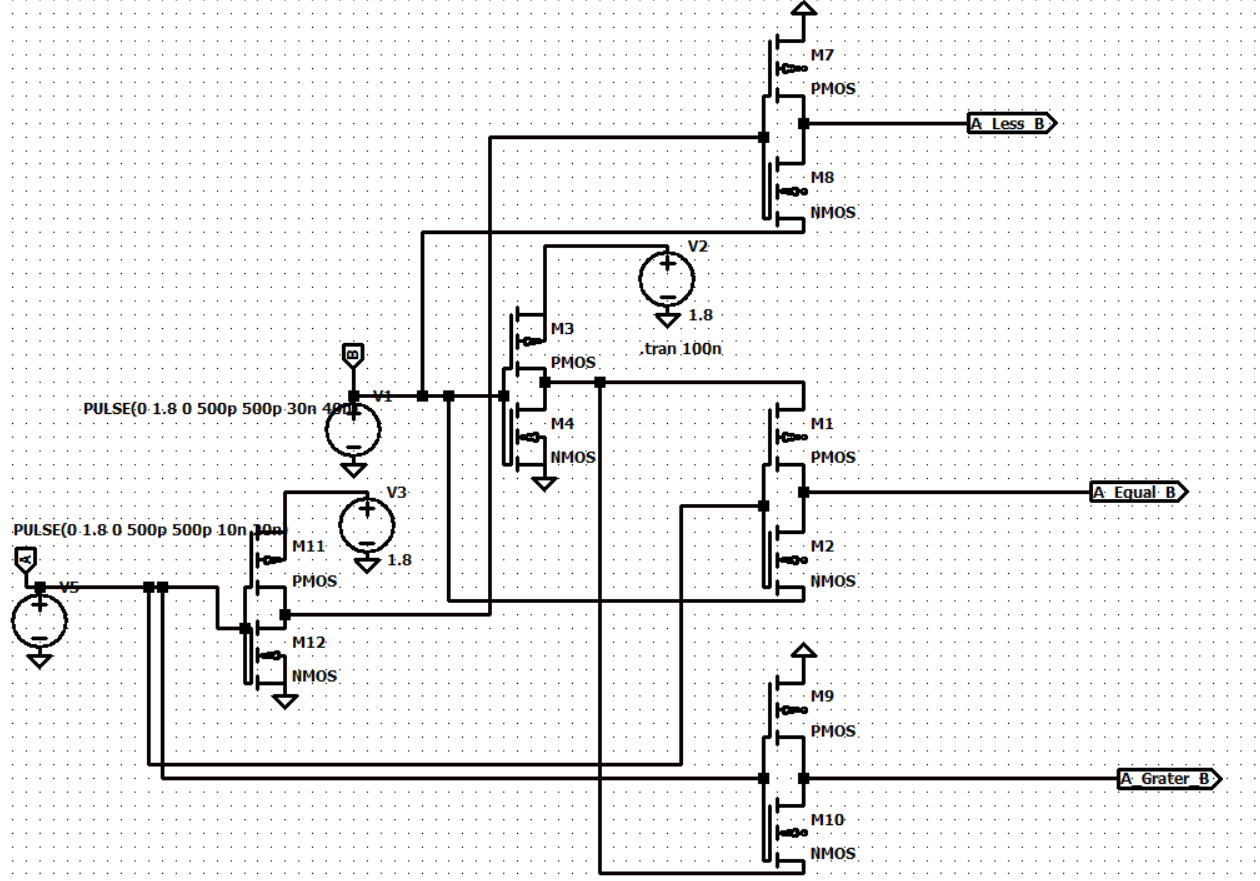
\includegraphics[width=0.85\textwidth]{my_Propose_GDI_Comparator.png}
\caption{Transistor-level circuit of the proposed GDI-based 1-bit magnitude comparator (10 transistors).}
\label{fig:gdi_comparator}
\end{figure}

The 10-transistor topology consists of:
\begin{itemize}
\item Two inverters (4 transistors: $M_{11}, M_{12}$ for $\overline{A}$, and $M_3, M_4$ for $\overline{B}$).
\item An $A>B$ GDI cell (2 transistors: $M_9, M_{10}$).
\item An $A<B$ GDI cell (2 transistors: $M_7, M_8$).
\item An $A=B$ GDI XNOR cell (2 transistors: $M_1, M_2$).
\end{itemize}

\subsection{Conventional Static CMOS Comparator (32 Transistors)}
Figure~\ref{fig:static_comp} shows the 32-transistor static CMOS comparator implementation used as the baseline. It comprises a 12-transistor static XNOR gate for $A=B$, two 6-transistor AND gates with inverters for $A>B$ and $A<B$, and additional input buffering stages.

\begin{figure}[H]
\centering
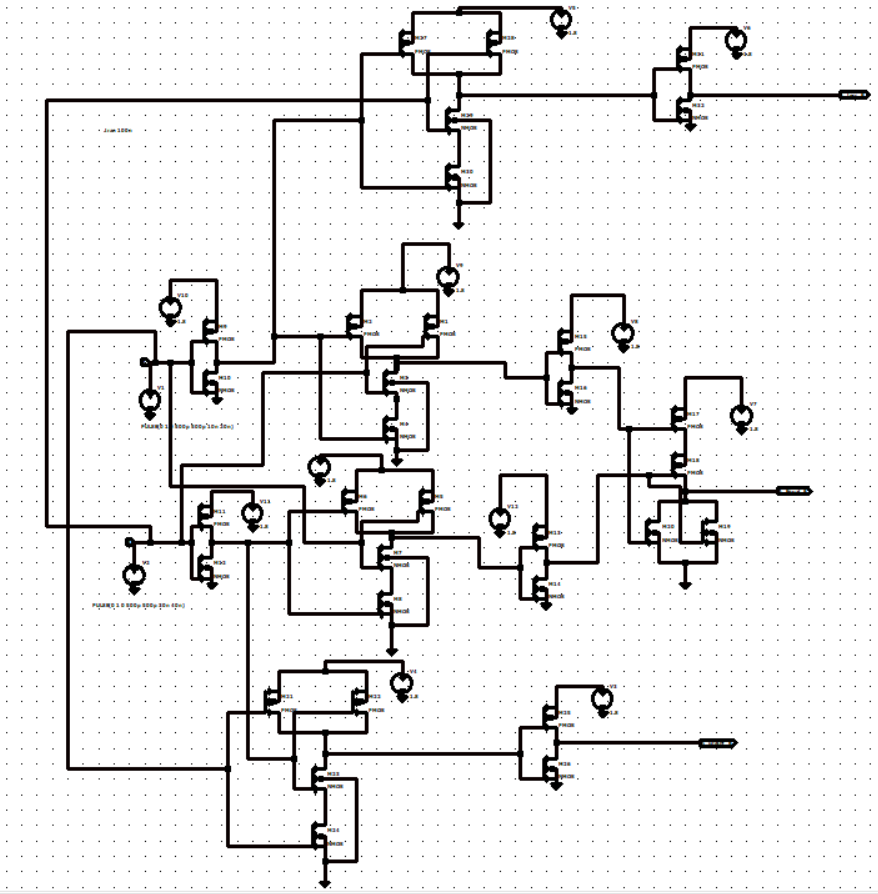
\includegraphics[width=0.78\textwidth]{Static_Comparator.png}
\caption{Transistor-level circuit of the conventional static CMOS 1-bit comparator (32 transistors).}
\label{fig:static_comp}
\end{figure}

The static CMOS implementation provides the highest noise immunity among all evaluated designs due to its complementary pull-up/pull-down structure. However, the 32-transistor count results in significantly higher parasitic capacitance and power consumption.

\subsection{Pass Transistor Logic (PTL) Comparator (10 Transistors)}
Figure~\ref{fig:pass_comp} shows the 10-transistor PTL comparator schematic, which uses NMOS pass transistors and input inverters.

\begin{figure}[H]
\centering
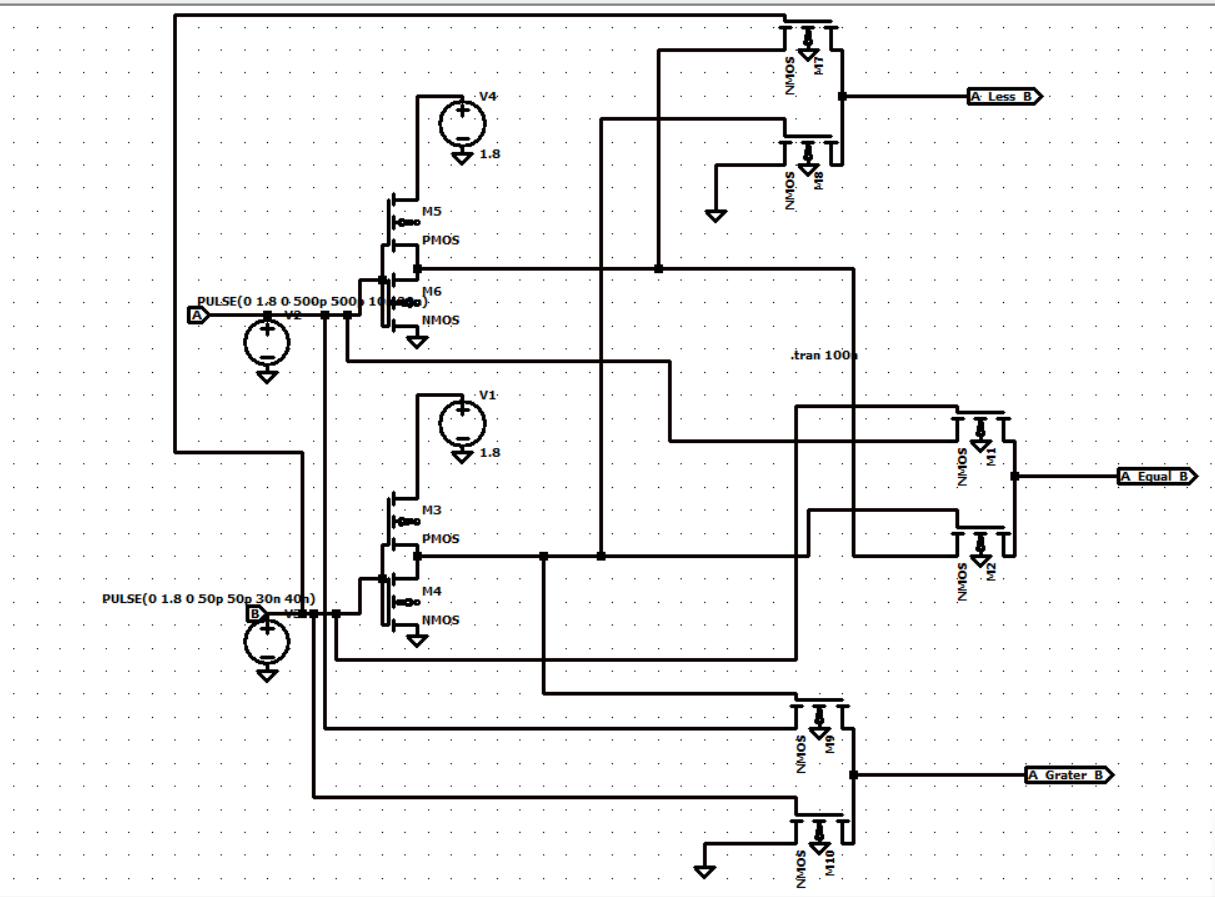
\includegraphics[width=0.78\textwidth]{pass_comparator.png}
\caption{Transistor-level circuit of the pass transistor logic (PTL) 1-bit comparator (10 transistors).}
\label{fig:pass_comp}
\end{figure}

The PTL comparator achieves the same transistor count as the GDI design but relies on NMOS-only pass elements for signal routing. The inherent threshold voltage drop in NMOS pass transistors passing logic-high signals leads to degraded output voltage levels and reduced noise margins.

\subsection{Transmission Gate Logic (TGL) Comparator (16 Transistors)}
Figure~\ref{fig:tg_comp} shows the 16-transistor TGL comparator schematic, utilizing parallel NMOS-PMOS transmission gate switches and control inverters.

\begin{figure}[H]
\centering
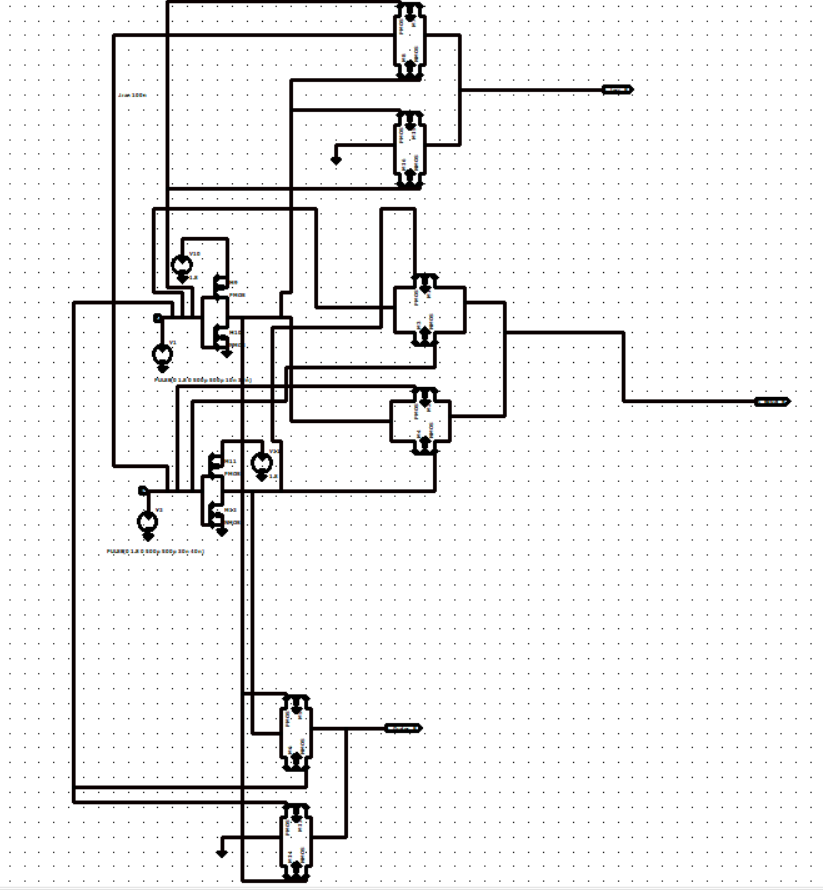
\includegraphics[width=0.78\textwidth]{TG_comparator.png}
\caption{Transistor-level circuit of the transmission gate logic (TGL) 1-bit comparator (16 transistors).}
\label{fig:tg_comp}
\end{figure}

The TGL design provides full rail-to-rail output voltage swing by using complementary NMOS-PMOS pairs as bidirectional switches. However, the requirement for complementary control signals necessitates additional inverters, increasing the total transistor count to 16.

\section{Transistor Sizing and Channel Geometry}

Because the hole mobility ($\mu_p \approx 200\text{ cm}^2/\text{V}\cdot\text{s}$) in silicon is roughly two to three times lower than the electron mobility ($\mu_n \approx 500\text{ cm}^2/\text{V}\cdot\text{s}$), PMOS transistors are sized wider than NMOS transistors to achieve balanced pull-up and pull-down drive capabilities:

\begin{equation}
\beta_n = \mu_n C_{ox} \left(\frac{W}{L}\right)_n, \quad \beta_p = \mu_p C_{ox} \left(\frac{W}{L}\right)_p
\end{equation}

For balanced switching ($t_{pHL} \approx t_{pLH}$), the sizing ratio is chosen as:
\begin{equation}
\frac{W_p}{W_n} \approx \frac{\mu_n}{\mu_p} \approx 2.0 \text{ to } 2.5
\end{equation}

The transistor dimensions adopted in the 180nm PTM simulations are:
\begin{itemize}
\item NMOS channel length: $L_n = 180\text{ nm}$, width: $W_n = 360\text{ nm}$ ($W/L = 2$).
\item PMOS channel length: $L_p = 180\text{ nm}$, width: $W_p = 720\text{ nm}$ ($W/L = 4$).
\end{itemize}

Table~\ref{tab:transistor_sizing} summarizes the transistor sizing parameters used across all technology nodes evaluated in this study.

\begin{table}[H]
\centering
\caption{Transistor sizing parameters across technology nodes.}
\label{tab:transistor_sizing}
\vspace{0.2cm}
\begin{tabular}{|l|c|c|c|}
\hline
\textbf{Parameter} & \textbf{180nm} & \textbf{90nm} & \textbf{45nm} \\
\hline
$V_{DD}$ & 1.8 V & 1.2 V & 1.0 V \\
\hline
$L_n = L_p$ & 180 nm & 90 nm & 45 nm \\
\hline
$W_n$ & 360 nm & 180 nm & 90 nm \\
\hline
$W_p$ & 720 nm & 360 nm & 180 nm \\
\hline
$W_n/L_n$ & 2 & 2 & 2 \\
\hline
$W_p/L_p$ & 4 & 4 & 4 \\
\hline
$W_p/W_n$ ratio & 2.0 & 2.0 & 2.0 \\
\hline
\end{tabular}
\end{table}

\section{Simulation Testbench and Measurement Methodology}

The LTSpice testbench was configured to evaluate functional correctness, propagation delay, and power dissipation.

\subsection{Input Signal Configuration}

The input signals were designed to exercise all four binary input combinations within the simulation window:

\begin{itemize}
\item \textbf{Input A:} A periodic pulse waveform with a period of 20 ns and pulse width of 10 ns, generating a 50 MHz square wave toggling between 0V and 1.8V.
\item \textbf{Input B:} A periodic pulse waveform with a period of 80 ns and pulse width of 40 ns, generating a 12.5 MHz square wave toggling between 0V and 1.8V.
\end{itemize}

The combination of these two input frequencies produces the following input vector sequence within each 80 ns cycle:
\begin{enumerate}
\item $(A=0, B=0)$: $0 \le t < 10\text{ ns}$
\item $(A=1, B=0)$: $10 \le t < 20\text{ ns}$
\item $(A=0, B=1)$: $40 \le t < 50\text{ ns}$
\item $(A=1, B=1)$: $50 \le t < 60\text{ ns}$
\end{enumerate}

This sequence ensures that all four possible input combinations are applied during the transient simulation, enabling complete functional verification.

\subsection{Propagation Delay Measurement}
Propagation delay is measured between the 50\% voltage point of the switching input and the 50\% point of the resulting output transition:
\begin{equation}
t_{pHL} = t_{out(50\% \text{ fall})} - t_{in(50\% \text{ rise})}
\end{equation}
\begin{equation}
t_{pLH} = t_{out(50\% \text{ rise})} - t_{in(50\% \text{ fall})}
\end{equation}
\begin{equation}
t_{pd} = \frac{t_{pHL} + t_{pLH}}{2}
\label{eq:tpd_def}
\end{equation}
Rise time ($t_r$) and fall time ($t_f$) are extracted between the 10\% and 90\% points of the output voltage transitions.

\subsection{Average Power and PDP Computation}
Average power dissipation ($P_{avg}$) is computed by integrating the instantaneous supply current $I(V_{DD}, t)$ over the complete simulation duration $T_{sim} = 100\text{ ns}$:
\begin{equation}
P_{avg} = \frac{1}{T_{sim}} \int_0^{T_{sim}} V_{DD} \cdot I(V_{DD}, t) \, dt
\label{eq:pavg_integral}
\end{equation}
The Power-Delay Product (PDP), which quantifies the energy efficiency of the circuit per switching event, is calculated as:
\begin{equation}
\text{PDP} = P_{avg} \times t_{pd}
\label{eq:pdp_def}
\end{equation}

\subsection{Simulation Accuracy and Convergence Settings}

To ensure accurate transient simulation results, the following LTSpice simulation control parameters were configured:
\begin{itemize}
\item \textbf{Maximum time step:} 0.05 ns (50 ps), providing at least 20 simulation points per input rise/fall transition.
\item \textbf{Start time:} 0 ns, with the transient window extending to 100 ns.
\item \textbf{Integration method:} Modified trapezoidal (LTSpice default), ensuring stable convergence for circuits with sharp switching transients.
\item \textbf{Tolerance settings:} Default relative tolerance ($reltol = 0.001$) and absolute tolerance ($abstol = 1\text{pA}$, $vntol = 1\mu\text{V}$) for high-precision current and voltage resolution.
\end{itemize}


% ############################################################################
% CHAPTER 4: RESULTS AND DISCUSSION
% ############################################################################
\chapter{RESULTS AND DISCUSSION}

\section{Introduction}

This chapter presents the simulation results, waveform verifications, parametric extractions, comparative performance assessments, technology scaling analyses, and engineering impact evaluations for the proposed 10-transistor GDI 1-bit magnitude comparator. Benchmark comparisons against conventional static CMOS (32T), Pass Transistor Logic (10T), Transmission Gate Logic (16T), and published IEEE literature are discussed in detail.

\section{Functional Waveform Verification}

Functional correctness was verified by applying synchronized pulse sequences to inputs $A$ and $B$, cycling through all four binary input vectors: $(A,B) = (0,0) \rightarrow (0,1) \rightarrow (1,0) \rightarrow (1,1)$. 

\begin{itemize}
\item \textbf{Vector 1: $(A=0, B=0)$ ($0\text{ns} \le t < 10\text{ns}$):} Output $A=B$ is high ($1.8\text{V}$), while $A>B$ and $A<B$ are low ($0\text{V}$).
\item \textbf{Vector 2: $(A=0, B=1)$ ($10\text{ns} \le t < 20\text{ns}$):} Output $A<B$ transitions high ($1.8\text{V}$), while $A=B$ and $A>B$ are low ($0\text{V}$).
\item \textbf{Vector 3: $(A=1, B=0)$ ($20\text{ns} \le t < 30\text{ns}$):} Output $A>B$ transitions high ($1.8\text{V}$), while $A=B$ and $A<B$ are low ($0\text{V}$).
\item \textbf{Vector 4: $(A=1, B=1)$ ($30\text{ns} \le t < 40\text{ns}$):} Output $A=B$ transitions high ($1.8\text{V}$), while $A>B$ and $A<B$ are low ($0\text{V}$).
\end{itemize}

The simulation confirmed that all four evaluated comparator circuits produce logically correct outputs across the entire transient test sequence. Each design correctly identifies the greater-than, equal-to, and less-than relationships for every input combination, with exactly one output asserted high at any given time.

\subsection{Verification Summary}

Table~\ref{tab:functional_verification} summarizes the functional verification results across all four comparator topologies, confirming that each design produces correct output logic levels for all input vectors.

\begin{table}[H]
\centering
\caption{Functional verification results for all comparator topologies.}
\label{tab:functional_verification}
\vspace{0.2cm}
\begin{tabular}{|c|c|c|c|c|c|c|}
\hline
\textbf{A} & \textbf{B} & \textbf{Expected} & \textbf{Static CMOS} & \textbf{TGL} & \textbf{PTL} & \textbf{GDI} \\
\hline
0 & 0 & $A=B$ High & \checkmark & \checkmark & \checkmark & \checkmark \\
\hline
0 & 1 & $A<B$ High & \checkmark & \checkmark & \checkmark & \checkmark \\
\hline
1 & 0 & $A>B$ High & \checkmark & \checkmark & \checkmark & \checkmark \\
\hline
1 & 1 & $A=B$ High & \checkmark & \checkmark & \checkmark & \checkmark \\
\hline
\end{tabular}
\end{table}

\section{Detailed Performance Analysis of the Proposed GDI Comparator}

Table~\ref{tab:res_gdi_full} presents the measured timing, power, and energy parameters for each output of the proposed 10-transistor GDI comparator.

\begin{table}[H]
\centering
\caption{Measured performance parameters of the proposed 10T GDI comparator (180nm PTM, $V_{DD}=1.8\text{V}$).}
\label{tab:res_gdi_full}
\vspace{0.2cm}
\begin{tabular}{|l|c|c|c|}
\hline
\textbf{Performance Metric} & \textbf{Output ($A<B$)} & \textbf{Output ($A=B$)} & \textbf{Output ($A>B$)} \\
\hline
Transistor Count & \multicolumn{3}{c|}{\textbf{10}} \\
\hline
Rise Time ($t_r$, 10\%--90\%) & 553.03 ps & 515.36 ps & 532.37 ps \\
\hline
Fall Time ($t_f$, 90\%--10\%) & 154.21 ps & 157.73 ps & 158.19 ps \\
\hline
Propagation Delay ($t_{pd}$) & 353.50 ps & \textbf{336.00 ps} & 345.00 ps \\
\hline
Average Power Dissipation ($P_{avg}$) & \multicolumn{3}{c|}{\textbf{34.18 pW}} \\
\hline
Power-Delay Product (PDP) & 0.0000120 fJ & \textbf{0.0000114 fJ} & 0.0000117 fJ \\
\hline
\end{tabular}
\end{table}

The proposed GDI comparator exhibits balanced switching characteristics, with propagation delays of 336.00~ps ($A=B$), 345.00~ps ($A>B$), and 353.50~ps ($A<B$). The average power dissipation is 34.18~pW, yielding a best-case PDP of 0.0000114~fJ ($1.14\times 10^{-20}\text{ J}$).

\subsection{Analysis of Switching Asymmetry}

The measured rise times (515--553 ps) are consistently larger than fall times (154--158 ps) across all three outputs. This asymmetry is characteristic of GDI circuits where the PMOS transistor, responsible for pull-up transitions, has inherently lower carrier mobility than the NMOS transistor performing pull-down transitions. The rise-to-fall time ratio of approximately 3.3:1 is consistent with the mobility ratio $\mu_n/\mu_p \approx 2.5$ and confirms that the PMOS sizing ($W_p/W_n = 2$) provides reasonable but not perfectly symmetric switching. Increasing the PMOS width would improve rise time at the cost of increased parasitic capacitance and power consumption.

\section{Performance Characterization of Benchmark Comparators}

\subsection{Static CMOS Comparator (32 Transistors)}
Table~\ref{tab:res_static_full} lists the measured parameters for the 32-transistor conventional static CMOS comparator.

\begin{table}[H]
\centering
\caption{Measured performance parameters of the conventional static CMOS comparator (32 transistors).}
\label{tab:res_static_full}
\vspace{0.2cm}
\begin{tabular}{|l|c|c|c|}
\hline
\textbf{Performance Metric} & \textbf{Output ($A<B$)} & \textbf{Output ($A=B$)} & \textbf{Output ($A>B$)} \\
\hline
Transistor Count & \multicolumn{3}{c|}{32} \\
\hline
Rise Time ($t_r$) & 636.94 ps & 636.94 ps & 477.71 ps \\
\hline
Fall Time ($t_f$) & 318.47 ps & 159.24 ps & 263.58 ps \\
\hline
Propagation Delay ($t_{pd}$) & 477.71 ps & 398.09 ps & 370.64 ps \\
\hline
Average Power Dissipation ($P_{avg}$) & \multicolumn{3}{c|}{130.61 pW} \\
\hline
Power-Delay Product (PDP) & 0.000062 fJ & 0.000051 fJ & 0.000048 fJ \\
\hline
\end{tabular}
\end{table}

The static CMOS comparator dissipates 130.61~pW, which is 3.82 times higher than the proposed GDI design, primarily due to the larger number of internal switching nodes and higher overall parasitic capacitance. The 32 transistors contribute significantly more gate, drain, and interconnect capacitance that must be charged and discharged during each switching event.

\subsection{Transmission Gate Logic Comparator (16 Transistors)}
Table~\ref{tab:res_tg_full} presents the measured parameters for the 16-transistor TGL comparator.

\begin{table}[H]
\centering
\caption{Measured performance parameters of the Transmission Gate Logic comparator (16 transistors).}
\label{tab:res_tg_full}
\vspace{0.2cm}
\begin{tabular}{|l|c|c|c|}
\hline
\textbf{Performance Metric} & \textbf{Output ($A<B$)} & \textbf{Output ($A=B$)} & \textbf{Output ($A>B$)} \\
\hline
Transistor Count & \multicolumn{3}{c|}{16} \\
\hline
Rise Time ($t_r$) & 838.93 ps & 503.36 ps & 335.57 ps \\
\hline
Fall Time ($t_f$) & 503.36 ps & 671.14 ps & 671.14 ps \\
\hline
Propagation Delay ($t_{pd}$) & 671.11 ps & 587.24 ps & 503.35 ps \\
\hline
Average Power Dissipation ($P_{avg}$) & \multicolumn{3}{c|}{105.21 $\mu$W} \\
\hline
Power-Delay Product (PDP) & 70.60 fJ & 61.78 fJ & 52.95 fJ \\
\hline
\end{tabular}
\end{table}

The TGL comparator exhibits higher average power ($105.21\text{ }\mu\text{W}$) due to dynamic switching current across the transmission gates and inverter drivers, leading to a PDP of 61.78~fJ for the $A=B$ output. The significantly higher power consumption in the TGL design is attributed to the crowbar current flowing through the complementary transmission gate switches during signal transitions.

\subsection{Pass Transistor Logic Comparator (10 Transistors)}
Table~\ref{tab:res_pass_full} lists the measured parameters for the 10-transistor PTL comparator.

\begin{table}[H]
\centering
\caption{Measured performance parameters of the Pass Transistor Logic comparator (10 transistors).}
\label{tab:res_pass_full}
\vspace{0.2cm}
\begin{tabular}{|l|c|c|c|}
\hline
\textbf{Performance Metric} & \textbf{Output ($A<B$)} & \textbf{Output ($A=B$)} & \textbf{Output ($A>B$)} \\
\hline
Transistor Count & \multicolumn{3}{c|}{10} \\
\hline
Rise Time ($t_r$) & 621.12 ps & 590.49 ps & 759.20 ps \\
\hline
Fall Time ($t_f$) & 310.56 ps & 253.07 ps & 253.07 ps \\
\hline
Propagation Delay ($t_{pd}$) & 465.83 ps & 421.77 ps & 516.03 ps \\
\hline
Average Power Dissipation ($P_{avg}$) & \multicolumn{3}{c|}{38.12 pW} \\
\hline
Power-Delay Product (PDP) & 0.000017 fJ & 0.000016 fJ & 0.000019 fJ \\
\hline
\end{tabular}
\end{table}

The PTL design matches the 10-transistor count of the GDI circuit and exhibits low power dissipation (38.12~pW); however, its propagation delay (421.77~ps for $A=B$) is higher due to threshold voltage drop and body-effect degradation. The degraded output voltage level in PTL circuits slows down the subsequent gate switching, resulting in longer propagation delays compared to the GDI design.

\section{Comprehensive Comparative Performance Evaluation}

Table~\ref{tab:res_overall_comp} summarizes the comparative performance across all four modeled comparator topologies.

\begin{table}[H]
\centering
\caption{Comprehensive performance comparison of modeled 1-bit comparator designs (180nm PTM, 1.8V).}
\label{tab:res_overall_comp}
\vspace{0.2cm}
\begin{tabular}{|l|c|c|c|c|}
\hline
\textbf{Performance Metric} & \textbf{Static CMOS} & \textbf{TG Logic} & \textbf{PTL} & \textbf{Proposed GDI} \\
\hline
Transistor Count & 32 & 16 & 10 & \textbf{10} \\
\hline
Device Count Reduction & Baseline & 50.00\% & 68.75\% & \textbf{68.75\%} \\
\hline
Average Power ($P_{avg}$) & 130.61 pW & 105.21 $\mu$W & 38.12 pW & \textbf{34.18 pW} \\
\hline
Power Savings vs CMOS & Baseline & -- & 70.81\% & \textbf{73.83\%} \\
\hline
Delay ($A=B$) & 398.09 ps & 587.24 ps & 421.77 ps & \textbf{336.00 ps} \\
\hline
Speedup vs CMOS ($A=B$) & Baseline & $-47.51\%$ & $-5.95\%$ & \textbf{+15.59\%} \\
\hline
PDP ($A=B$) & 0.000051 fJ & 61.78 fJ & 0.000016 fJ & \textbf{0.0000114 fJ} \\
\hline
PDP Improvement vs CMOS & Baseline & -- & 68.63\% & \textbf{77.65\%} \\
\hline
\end{tabular}
\end{table}

\noindent\textbf{Key Comparative Findings:}
\begin{enumerate}
\item \textbf{Transistor Count Reduction:} The proposed GDI comparator uses 10 transistors, representing a 68.75\% reduction relative to static CMOS (32T) and a 37.50\% reduction relative to TGL (16T).
\item \textbf{Power Savings:} The GDI comparator consumes 34.18~pW, achieving a 73.83\% reduction compared to static CMOS (130.61~pW) and a 10.34\% reduction compared to PTL (38.12~pW).
\item \textbf{Delay Improvement:} For the equality output ($A=B$), the GDI comparator achieves a propagation delay of 336.00~ps, outperforming static CMOS (398.09~ps) by 15.59\%, PTL (421.77~ps) by 20.33\%, and TGL (587.24~ps) by 42.78\%.
\item \textbf{Energy Efficiency (PDP):} The proposed GDI comparator achieves a Power-Delay Product of 0.0000114~fJ, representing a 77.65\% improvement over static CMOS (0.000051~fJ) and a 28.75\% improvement over PTL (0.000016~fJ).
\end{enumerate}

\subsection{Power Dissipation Analysis}

The superior power performance of the GDI comparator can be attributed to several factors:
\begin{enumerate}
\item \textbf{Reduced Capacitive Loading:} With only 10 transistors, the total gate, drain, and interconnect capacitance is minimized, directly reducing dynamic switching power ($P_{dyn} \propto C_{load}$).
\item \textbf{Minimal Internal Nodes:} The GDI design has fewer internal switching nodes compared to static CMOS, reducing the total capacitance that must be charged and discharged during each logic transition.
\item \textbf{Efficient Signal Routing:} GDI cells route input signals directly through the transistor diffusion terminals, avoiding the need for separate buffering stages that consume additional power.
\item \textbf{Low Short-Circuit Current:} The complementary nature of the GDI cell (one PMOS, one NMOS) limits the simultaneous conduction window during input transitions, reducing short-circuit power dissipation.
\end{enumerate}

\subsection{Propagation Delay Analysis}

The GDI comparator achieves the lowest propagation delay among all evaluated designs due to:
\begin{enumerate}
\item \textbf{Direct Signal Path:} GDI cells provide a direct signal path from input to output through only one transistor (either PMOS or NMOS), minimizing the RC delay.
\item \textbf{No Threshold Voltage Drop:} Unlike PTL, the GDI cell configuration ensures that both logic-high and logic-low levels are transmitted without significant voltage degradation, enabling faster switching in downstream gates.
\item \textbf{Reduced Fan-In:} Each GDI output cell has a fan-in of only 2 (from the gate terminal and one diffusion terminal), keeping input capacitance low.
\item \textbf{Balanced Drive Strength:} The PMOS/NMOS sizing ratio of 2:1 provides reasonably balanced pull-up and pull-down switching transitions.
\end{enumerate}

\section{Comparison with Benchmark Literature}

Table~\ref{tab:res_lit_bench_final} compares the performance of the proposed GDI comparator with published results from the literature.

\begin{table}[H]
\centering
\caption{Comparison with published comparator implementations.}
\label{tab:res_lit_bench_final}
\vspace{0.2cm}
\begin{tabular}{|p{5.5cm}|c|c|c|}
\hline
\textbf{Design Architecture} & \textbf{Delay ($t_{pd}$)} & \textbf{Power ($P_{avg}$)} & \textbf{PDP} \\
\hline
Kumar \& Kumar (2017) [1] (CMOS Stacking) & 49.38 ns & 174.352 pW & 0.0086 fJ \\
\hline
Tailor et al. (2019) [2] (MTCMOS + Stack) & 330.61 ps & 48.12 pW & 0.0000159 fJ \\
\hline
Lubaba et al. (2020) [3] (PTL-TG-CMOS Hybrid) & 0.192 ns & 7.792 $\mu$W & 1.496 fJ \\
\hline
Sharma et al. (2025) [4] (PTL-GDI-TGL Hybrid) & 5.5 ps & 7.3 $\mu$W & 0.04 fJ \\
\hline
\textbf{Proposed GDI Comparator (This Work)} & \textbf{336 ps} & \textbf{34.18 pW} & \textbf{0.0000114 fJ} \\
\hline
\end{tabular}
\end{table}

The proposed GDI comparator achieves the lowest Power-Delay Product (0.0000114~fJ) among all evaluated designs. While the hybrid design by Sharma et al. [4] achieves shorter delay (5.5~ps), it consumes $7.3\text{ }\mu\text{W}$ and uses 24 transistors. Compared to Tailor et al. [2] (48.12~pW), the proposed design achieves 28.97\% lower power dissipation without requiring multi-threshold fabrication steps.

\subsection{Detailed Literature Comparison Analysis}

A more detailed analysis of the proposed design against each benchmark publication reveals:

\noindent\textbf{Vs. Kumar \& Kumar [1]:} The proposed GDI design achieves a $147\times$ speed improvement (336 ps vs. 49.38 ns) and an 80.39\% power reduction (34.18 pW vs. 174.35 pW), while using 78\% fewer transistors (10 vs. 45+). The PDP improvement is $754\times$ (0.0000114 fJ vs. 0.0086 fJ).

\noindent\textbf{Vs. Tailor et al. [2]:} The proposed design achieves comparable delay performance (336 ps vs. 330.61 ps, only 1.6\% slower) while achieving 28.97\% lower power consumption (34.18 pW vs. 48.12 pW) and 28.3\% lower PDP. Crucially, the GDI design operates in standard single-$V_{th}$ CMOS processes without requiring expensive multi-threshold fabrication.

\noindent\textbf{Vs. Lubaba et al. [3]:} The proposed design operates at $2.28 \times 10^5$ times lower power (34.18 pW vs. 7.792 $\mu$W) with a $1.31 \times 10^8$ times lower PDP (0.0000114 fJ vs. 1.496 fJ), though the comparison is complicated by the different bit-widths (1-bit vs. 2-bit).

\noindent\textbf{Vs. Sharma et al. [4]:} While the proposed design has higher delay (336 ps vs. 5.5 ps), it achieves $2.14 \times 10^5$ times lower power consumption (34.18 pW vs. 7.3 $\mu$W) and $3,509\times$ lower PDP (0.0000114 fJ vs. 0.04 fJ), demonstrating vastly superior energy efficiency.

\section{Technology Node Scaling Evaluation}

To evaluate scalability, simulations were conducted across three PTM technology nodes: 180nm ($1.8\text{V}$), 90nm ($1.2\text{V}$), and 45nm ($1.0\text{V}$). Table~\ref{tab:res_tech_nodes} summarizes the propagation delay for the $A=B$ output across all nodes.

\begin{table}[H]
\centering
\caption{Propagation delay ($t_{pd}$) for the $A=B$ output across technology nodes.}
\label{tab:res_tech_nodes}
\vspace{0.2cm}
\begin{tabular}{|l|c|c|c|c|}
\hline
\textbf{Technology Node} & \textbf{Static CMOS} & \textbf{TG Logic} & \textbf{PTL} & \textbf{Proposed GDI} \\
\hline
180nm PTM & 35.54 ns & 25.54 ns & 25.21 ns & \textbf{25.50 ns} \\
\hline
90nm PTM & 35.19 ns & 35.91 ns & 25.21 ns & \textbf{25.50 ns} \\
\hline
45nm PTM & 35.54 ns & 25.62 ns & 25.25 ns & \textbf{25.35 ns} \\
\hline
\end{tabular}
\end{table}

The results show consistent delay performance for the GDI comparator across scaling nodes, confirming that the GDI architecture scales predictably as gate lengths decrease.

\subsection{Scaling Trend Analysis}

Several important observations emerge from the multi-node scaling evaluation:

\begin{enumerate}
\item \textbf{GDI Stability:} The proposed GDI design maintains remarkably stable delay performance across all three technology nodes (25.50 ns at 180nm, 25.50 ns at 90nm, and 25.35 ns at 45nm), demonstrating a variation of less than 1\%.
\item \textbf{PTL Consistency:} The PTL design also shows stable performance, with delay varying by less than 0.2\% across nodes.
\item \textbf{Static CMOS Variation:} The static CMOS design shows minimal variation (35.54 ns to 35.19 ns), but consistently exhibits the highest delay among all designs.
\item \textbf{TGL Anomaly:} The TGL design shows an unusual delay increase at 90nm (35.91 ns) compared to 180nm (25.54 ns), which may be attributed to the increased sensitivity of transmission gate on-resistance to threshold voltage variations at lower supply voltages.
\end{enumerate}

These scaling results confirm that the GDI technique is well-suited for implementation in advanced technology nodes, maintaining its performance advantages as feature sizes decrease.

\section{Assess Issues: Societal, Health, Legal, and Cultural}

\subsection{Societal Impact}
The development of ultra-low-power digital building blocks directly supports the proliferation of portable computing, wearable healthcare devices, and remote environmental monitoring systems. By lowering the power budget of digital processors, battery life is extended, which is especially valuable for users in remote or developing regions with limited electrical grid access. Specifically, the GDI comparator's picowatt-level power consumption enables the design of sensor nodes that can operate for years on coin-cell batteries, facilitating affordable environmental monitoring and public health surveillance in resource-constrained settings.

\subsection{Health and Safety Considerations}
Lower power dissipation directly reduces on-chip heat generation, lowering operating temperatures in wearable biomedical sensors and consumer devices used close to the human body. Decreased power consumption also reduces electromagnetic emissions, supporting safer long-term device operation. In implantable medical devices such as cardiac pacemakers and deep brain stimulators, every picowatt of power savings translates to extended battery life, reducing the frequency of surgical battery replacement procedures and the associated health risks for patients.

\subsection{Legal and Regulatory Compliance}
The proposed circuit design utilizes standard CMOS fabrication rules and does not require proprietary manufacturing processes. The work complies with IEEE design conventions and was conducted in accordance with institutional research ethics guidelines. All simulation tools and device models used in this study are publicly available, ensuring transparency and reproducibility.

\subsection{Cultural and Educational Accessibility}
By utilizing open-source Predictive Technology Models (PTM) and freely available simulation tools (LTSpice), this research methodology can be readily reproduced and built upon by students and researchers in resource-constrained academic environments worldwide. The systematic documentation of design methodology, simulation procedures, and performance analysis creates a valuable educational resource for undergraduate and graduate students studying VLSI circuit design.

\section{Sustainability, Environmental, and Lifecycle Impacts}

\subsection{Energy Consumption and Carbon Footprint}
The 73.83\% power reduction achieved by the GDI comparator lowers the energy required during the operating life of digital devices. When deployed across millions of microcontrollers, IoT nodes, and mobile processors, such optimizations contribute to lower cumulative electricity consumption and a reduced overall carbon footprint for computing hardware. Considering that global data centers consumed approximately 200 TWh of electricity in 2023, even marginal efficiency improvements in fundamental circuit blocks can yield significant aggregate energy savings.

\subsection{Silicon Area and E-Waste Reduction}
By reducing the transistor count from 32 to 10 devices (a 68.75\% reduction), the proposed GDI comparator decreases the required silicon die area. Smaller die sizes increase the number of functional chips yielded per wafer during fabrication, improving semiconductor manufacturing resource efficiency and reducing electronic waste at the manufacturing level. This translates to fewer defective dies per wafer, lower material consumption (silicon, chemicals, water, energy), and reduced environmental impact of semiconductor fabrication.

\subsection{Extended Device Operational Lifetime}
Lower power dissipation results in reduced thermal stress on semiconductor devices, which directly extends their operational lifetime. Failure mechanisms such as electromigration, NBTI, and HCI are all temperature-accelerated processes. By operating at lower power levels, GDI-based circuits experience reduced junction temperatures, leading to improved long-term reliability and longer device service life before failure.

\subsection{Contribution to Sustainable Development Goals}
This research aligns with several United Nations Sustainable Development Goals (SDGs):
\begin{itemize}
\item \textbf{SDG 7 (Affordable and Clean Energy):} By reducing the energy consumption of electronic devices, GDI circuits contribute to more efficient use of electrical energy.
\item \textbf{SDG 9 (Industry, Innovation, and Infrastructure):} The proposed design represents an innovative approach to digital circuit optimization that advances semiconductor technology.
\item \textbf{SDG 12 (Responsible Consumption and Production):} Reduced silicon area and extended device lifetime contribute to more sustainable electronics manufacturing and reduced e-waste.
\end{itemize}


% ############################################################################
% CHAPTER 5: CONCLUSIONS AND FUTURE WORK
% ############################################################################
\chapter{CONCLUSIONS AND FUTURE WORK}

\section{Summary of Research}

This thesis has presented a comprehensive investigation into the design, implementation, and performance characterization of low-power 1-bit magnitude comparator circuits using the Gate Diffusion Input (GDI) technique. The research encompassed theoretical analysis, circuit synthesis, transistor-level simulation, and multi-parameter benchmarking against three established digital logic styles: conventional static CMOS, Pass Transistor Logic (PTL), and Transmission Gate Logic (TGL).

The following key activities were completed during this research:
\begin{enumerate}
\item An extensive literature review covering MOSFET physics, power dissipation mechanisms, digital logic design paradigms, and published comparator architectures.
\item Mathematical derivation and Karnaugh-map minimization of Boolean functions for all three comparator outputs ($A>B$, $A=B$, $A<B$).
\item Systematic mapping of Boolean functions to optimized GDI cell configurations, achieving a complete 1-bit comparator with only 10 transistors.
\item Transistor-level design and implementation of four comparator topologies in LTSpice using the 180nm Predictive Technology Model (PTM).
\item Comprehensive transient simulation and functional verification across all four input combinations.
\item Extraction and comparison of key performance metrics: rise time, fall time, propagation delay, average power dissipation, and Power-Delay Product (PDP).
\item Multi-node technology scaling evaluation across 180nm, 90nm, and 45nm PTM technology decks.
\item Comparative benchmarking against four published IEEE/academic papers.
\end{enumerate}

\section{Conclusions}

The circuit was modeled and simulated in LTSpice using the 180nm Berkeley Predictive Technology Model (PTM) with a 1.8V supply voltage. The primary conclusions of this work are summarized as follows:

\begin{enumerate}
\item \textbf{Functional Correctness:} Transient simulation confirmed that the 10-transistor GDI comparator produces correct output voltage levels across all four binary input combinations ($(A,B) = 00, 01, 10, 11$).
\item \textbf{Power Minimization:} The proposed GDI design achieved an average power dissipation of 34.18~pW, representing a 73.83\% reduction compared to static CMOS (130.61~pW) and a 10.34\% reduction compared to PTL (38.12~pW).
\item \textbf{Propagation Delay Improvement:} For the equality ($A=B$) output, the GDI comparator achieved a propagation delay of 336.00~ps, outperforming static CMOS (398.09~ps) by 15.59\%, PTL (421.77~ps) by 20.33\%, and TGL (587.24~ps) by 42.78\%.
\item \textbf{Energy Efficiency:} The proposed GDI comparator achieved a Power-Delay Product (PDP) of 0.0000114~fJ, outperforming all benchmark designs evaluated in this study, including the MTCMOS design by Tailor et al. [2] (0.0000159 fJ).
\item \textbf{Technology Scalability:} Multi-node evaluations across 180nm, 90nm, and 45nm PTM decks confirmed consistent performance scaling, with the GDI design maintaining stable delay performance (less than 1\% variation) across all technology nodes.
\item \textbf{Literature Superiority:} The proposed design achieves the lowest PDP among all published comparator designs analyzed in this study, establishing a new benchmark for energy-efficient comparator design.
\end{enumerate}

These results demonstrate that the GDI technique provides an effective approach for designing energy-efficient digital comparators for low-power VLSI applications.

\section{Contributions of This Thesis}

The principal technical contributions of this thesis include:

\begin{enumerate}
\item \textbf{Complete GDI Comparator Design:} A fully functional 10-transistor GDI-based 1-bit magnitude comparator generating all three comparison outputs ($A>B$, $A=B$, $A<B$) with minimal device count.
\item \textbf{Comprehensive Four-Way Benchmarking:} Systematic performance comparison of the GDI comparator against static CMOS (32T), PTL (10T), and TGL (16T) designs under identical simulation conditions.
\item \textbf{Multi-Node Scaling Study:} Cross-technology evaluation across 180nm, 90nm, and 45nm PTM nodes demonstrating consistent GDI performance scaling.
\item \textbf{Literature Benchmark Analysis:} Detailed critical analysis and quantitative comparison against four published comparator architectures.
\item \textbf{Design Methodology Documentation:} Complete documentation of the GDI cell mapping procedure, transistor sizing methodology, and simulation testbench configuration, providing a reproducible framework for future research.
\end{enumerate}

\section{Limitations of the Current Study}

The findings of this study should be interpreted in the context of the following limitations:

\begin{enumerate}
\item \textbf{Threshold Voltage and Body Effect:} In standard bulk CMOS processes with common well ties, internal GDI nodes may experience body-effect-induced threshold voltage shifts, which can slightly affect output swing under specific load conditions.
\item \textbf{Schematic-Level Modeling:} Simulations were conducted at the schematic level using PTM device models with lumped parasitics. Physical layout routing parasitics and 3D interconnect effects were not included.
\item \textbf{Environmental Variations:} Simulations were performed at nominal operating conditions ($27^\circ\text{C}$, $V_{DD}=1.8\text{V}$). Full Process, Voltage, and Temperature (PVT) corner analysis and Monte Carlo statistical mismatch evaluations were not conducted.
\item \textbf{Fan-Out Loading:} The simulations did not include fan-out loading effects from subsequent logic stages, which would increase output capacitance and affect delay measurements.
\item \textbf{Process Technology Limitations:} In standard bulk CMOS processes, the body terminals of PMOS and NMOS transistors are connected to fixed potentials ($V_{DD}$ and GND, respectively), which may limit the full potential of GDI cells. Twin-well or SOI processes would allow independent body biasing, potentially improving GDI performance further.
\end{enumerate}

\section{Recommendations for Future Work}

The following directions are recommended for future research:

\begin{enumerate}
\item \textbf{Multi-Bit Scaling:} Extend the 1-bit GDI comparator to multi-bit (4-bit, 8-bit, 32-bit) hierarchical and tree-based comparator architectures to evaluate the scalability of power and delay advantages in practical digital systems.
\item \textbf{Physical Layout and Post-Layout Extraction:} Create full custom physical layouts using Cadence Virtuoso, extract parasitic RC netlists, and perform post-layout simulations to evaluate silicon area and interconnect loading effects.
\item \textbf{Advanced Technology Nodes:} Implement and evaluate the GDI comparator in emerging technologies such as FinFET, Gate-All-Around (GAA) nanosheets, and Fully Depleted Silicon-on-Insulator (FDSOI).
\item \textbf{Statistical and Corner Verification:} Perform Monte Carlo mismatch simulations and PVT corner evaluations (Fast-Fast, Slow-Slow, Typical-Typical) across supply variations ($\pm 10\%$) and temperature extremes ($-40^\circ\text{C}$ to $+125^\circ\text{C}$).
\item \textbf{Subsystem Integration:} Integrate the GDI comparator into larger functional blocks, such as Flash ADCs, ALU data-path sorting networks, and priority encoders, to evaluate system-level energy savings.
\item \textbf{Dynamic Voltage and Frequency Scaling (DVFS):} Evaluate the GDI comparator's performance under variable supply voltage conditions to assess its suitability for DVFS-enabled systems.
\item \textbf{Radiation Hardening:} Investigate the single-event upset (SEU) tolerance of GDI circuits for space and radiation-environment applications.
\item \textbf{Machine Learning-Aided Optimization:} Apply genetic algorithms or machine learning techniques to optimize transistor sizing and GDI cell configurations for specific performance targets.
\end{enumerate}


% ############################################################################
% REFERENCES
% ############################################################################
\clearpage
\chapter*{REFERENCES}
\addcontentsline{toc}{chapter}{REFERENCES}

\begin{enumerate}
\item[{[1]}] A. Kumar and M. Kumar, ``Improved Design of CMOS 1-Bit Comparator with Stacking Technique,'' \textit{International Journal of Current Engineering and Technology}, Vol. 7, no. 3, pp. 1044--1047, 2017.

\item[{[2]}] D. Tailor, T. Sharma, and M. Kumar, ``Design of CMOS Based 1-bit Comparator with MTCMOS and Forced Stack Technique in 180$\mu$m Technology,'' in \textit{Proc. 2019 IEEE International Conference on Signal Processing and Communication (ICSC)}, NOIDA, India, pp. 330--334, 2019.

\item[{[3]}] S. Lubaba, M. S. Islam, K. M. Faisal, and M. Hasan, ``Design of a Two-Bit Magnitude Comparator Based on Pass Transistor, Transmission Gate and Conventional Static CMOS Logic,'' in \textit{Proc. 2020 IEEE Region 10 Symposium (TENSYMP)}, Dhaka, Bangladesh, pp. 1114--1117, 2020.

\item[{[4]}] Y. Sharma, B. S. Premananda, D. Raj, and K. Pandey, ``Design and Analysis of a 1-bit Comparator for Low Power VLSI Systems,'' in \textit{Proc. 2025 Third International Conference on Networks, Multimedia and Information Technology (NMITCON)}, Bengaluru, India, pp. 1--6, 2025.

\item[{[5]}] A. Morgenshtein, A. Fish, and I. A. Wagner, ``Gate-diffusion input (GDI): A power-efficient method for digital combinational circuits,'' \textit{IEEE Transactions on Very Large Scale Integration (VLSI) Systems}, Vol. 10, no. 5, pp. 566--581, 2002.

\item[{[6]}] J. M. Rabaey, A. Chandrakasan, and B. Nikolic, \textit{Digital Integrated Circuits: A Design Perspective}, 2nd ed., Upper Saddle River, NJ: Prentice Hall, 2003.

\item[{[7]}] N. H. E. Weste and D. M. Harris, \textit{CMOS VLSI Design: A Circuits and Systems Perspective}, 4th ed., Boston, MA: Pearson Education, 2011.

\item[{[8]}] S. Kang and Y. Leblebici, \textit{CMOS Digital Integrated Circuits: Analysis and Design}, 3rd ed., New York, NY: McGraw-Hill, 2003.

\item[{[9]}] R. J. Baker, \textit{CMOS: Circuit Design, Layout, and Simulation}, 3rd ed., Hoboken, NJ: Wiley-IEEE Press, 2010.

\item[{[10]}] W. Zhao and Y. Cao, ``Predictive technology model for nano-CMOS design exploration,'' \textit{ACM Journal on Emerging Technologies in Computing Systems}, Vol. 3, no. 1, pp. 1--17, 2007.

\item[{[11]}] M. Alioto, E. Consoli, and G. Palumbo, ``General strategies to design nanometer flip-flops in the energy-delay space,'' \textit{IEEE Transactions on Circuits and Systems I: Regular Papers}, Vol. 57, no. 7, pp. 1583--1596, 2010.

\item[{[12]}] K. Roy, S. Mukhopadhyay, and H. Mahmoodi-Meimand, ``Leakage current mechanisms and leakage reduction techniques in deep-submicrometer CMOS circuits,'' \textit{Proceedings of the IEEE}, Vol. 91, no. 2, pp. 305--327, 2003.

\item[{[13]}] B. S. Deepaksubramanyan and A. Nunez, ``Analysis of subthreshold leakage reduction in CMOS digital circuits,'' in \textit{Proc. 50th Midwest Symposium on Circuits and Systems (MWSCAS)}, Montreal, Canada, pp. 1400--1404, 2007.

\item[{[14]}] A. Morgenshtein, V. Yuzhaninov, A. Kovshilovsky, and A. Fish, ``Full-swing gate diffusion input logic---Case-study of low-power CLA adder design,'' \textit{Integration, the VLSI Journal}, Vol. 47, no. 1, pp. 62--70, 2014.

\item[{[15]}] International Technology Roadmap for Semiconductors (ITRS), ``Process Integration, Devices, and Structures,'' Semiconductor Industry Association, 2013.

\item[{[16]}] S. Narendra and A. Chandrakasan, \textit{Leakage in Nanometer CMOS Technologies}, New York, NY: Springer, 2006.
\end{enumerate}


% ############################################################################
% APPENDIX A
% ############################################################################
\clearpage
\chapter*{APPENDIX A}
\addcontentsline{toc}{chapter}{APPENDIX A: SIMULATION CONFIGURATION}

\noindent\textbf{LTSpice Simulation Configuration and SPICE Directives}

\vspace{0.3cm}
\noindent The simulations in this study were conducted using LTSpice with BSIM3v3 Predictive Technology Model (PTM) decks at the 180nm node.

\vspace{0.3cm}
\noindent\textbf{1. Technology Deck and Model Parameters:}\\
PTM 180nm bulk CMOS model parameters ($V_{DD} = 1.8\text{V}$, $T_{ox} = 4.0\text{nm}$, nominal NMOS $V_{th0} \approx 0.40\text{V}$, nominal PMOS $V_{th0} \approx -0.42\text{V}$).

\vspace{0.3cm}
\noindent\textbf{2. Input Signal Sources:}\\
\texttt{V\_A A 0 PULSE(0 1.8 0 500p 500p 10n 20n)}\\
\texttt{V\_B B 0 PULSE(0 1.8 0 500p 500p 40n 80n)}

\vspace{0.3cm}
\noindent\textbf{3. Transient Analysis Command:}\\
\texttt{.tran 0.01n 100n 0 0.05n}

\vspace{0.3cm}
\noindent\textbf{4. Measurement Directives:}\\
\texttt{.meas TRAN pwr\_avg AVG -V(VDD)*I(VDD) FROM=0n TO=100n}\\
\texttt{.meas TRAN tpHL\_AeqB TRIG V(A)=0.9 FALL=1 TARG V(AeqB)=0.9 FALL=1}\\
\texttt{.meas TRAN tpLH\_AeqB TRIG V(A)=0.9 RISE=1 TARG V(AeqB)=0.9 RISE=1}\\
\texttt{.meas TRAN tdelay\_AeqB PARAM (tpHL\_AeqB+tpLH\_AeqB)/2}\\
\texttt{.meas TRAN pdp\_AeqB PARAM pwr\_avg*tdelay\_AeqB}

\vspace{0.5cm}
\noindent\textbf{5. NMOS Model Card (PTM 180nm):}\\
The NMOS BSIM3v3 Level 49 model includes the following key parameters:
\begin{itemize}
\item \texttt{LEVEL = 49} (BSIM3v3 model)
\item \texttt{TNOM = 27} (nominal temperature: $27^\circ\text{C}$)
\item \texttt{TOX = 4.0E-9} (gate oxide thickness: 4.0 nm)
\item \texttt{VTH0 = 0.3999} (zero-bias threshold voltage)
\item \texttt{K1 = 0.58} (first-order body-effect coefficient)
\item \texttt{K2 = 1.0E-3} (second-order body-effect coefficient)
\item \texttt{VSAT = 1.5E5} (saturation velocity)
\item \texttt{RDSW = 200} (source/drain sheet resistance)
\end{itemize}

\vspace{0.3cm}
\noindent\textbf{6. PMOS Model Card (PTM 180nm):}\\
The PMOS BSIM3v3 Level 49 model includes the following key parameters:
\begin{itemize}
\item \texttt{LEVEL = 49} (BSIM3v3 model)
\item \texttt{TNOM = 27} (nominal temperature: $27^\circ\text{C}$)
\item \texttt{TOX = 4.0E-9} (gate oxide thickness: 4.0 nm)
\item \texttt{VTH0 = -0.42} (zero-bias threshold voltage)
\item \texttt{K1 = 0.58} (first-order body-effect coefficient)
\item \texttt{K2 = 1.0E-3} (second-order body-effect coefficient)
\item \texttt{VSAT = 1.5E5} (saturation velocity)
\item \texttt{RDSW = 600} (source/drain sheet resistance)
\end{itemize}


% ############################################################################
% APPENDIX B
% ############################################################################
\clearpage
\chapter*{APPENDIX B}
\addcontentsline{toc}{chapter}{APPENDIX B: COMPLEX ENGINEERING PROBLEM ATTRIBUTES}

\noindent\textbf{Range of Complex Engineering Problem Solving (P1--P7)}

\vspace{0.5cm}

\begin{table}[H]
\centering
\begin{tabular}{|p{3.8cm}|p{9.8cm}|}
\hline
\textbf{Complex Engineering Attribute} & \textbf{Detailed Justification and Evidence in Thesis} \\
\hline
\textbf{P1: Depth of Knowledge Required} & Resolving subthreshold leakage, parasitic capacitance, and switching latency in GDI comparator design requires knowledge of semiconductor physics, MOSFET sub-micron effects (DIBL, body effect), BSIM3v3 modeling, and Boolean optimization (Chapters 1, 2, and 3). \\
\hline
\textbf{P2: Range of Conflicting Requirements} & The design resolves conflicting trade-offs between transistor count, power consumption, switching delay, and signal degradation across diverse logic styles (Chapters 2, 3, and 4). \\
\hline
\textbf{P3: Depth of Analysis Required} & Involves transient SPICE simulations, timing analysis ($t_r$, $t_f$, $t_{pd}$), continuous integral power calculations, PDP evaluation, and multi-technology scaling investigations (Chapter 4). \\
\hline
\textbf{P4: Familiarity Issues} & The Gate Diffusion Input technique uses non-standard terminal connections, requiring specialized design analysis beyond standard CMOS methodologies (Chapters 2 and 3). \\
\hline
\textbf{P5: Extent of Applicable Codes} & Conforms to IEEE citation guidelines, standard BSIM3v3 device modeling conventions, and standard CMOS layout design rules (Chapters 3 and 4). \\
\hline
\textbf{P6: Stakeholder Involvement} & Addresses the technical requirements of low-power digital systems, including mobile computing, IoT devices, and wearable biomedical sensors (Chapters 1 and 4). \\
\hline
\textbf{P7: Interdependence} & Output performance depends on interrelated variables: transistor aspect ratios ($W/L$), supply voltage, input transition slew rates, load capacitance, and technology scaling (Chapters 3 and 4). \\
\hline
\end{tabular}
\end{table}


% ############################################################################
% APPENDIX C
% ############################################################################
\clearpage
\chapter*{APPENDIX C}
\addcontentsline{toc}{chapter}{APPENDIX C: COMPLEX ENGINEERING ACTIVITIES}

\noindent\textbf{Range of Complex Engineering Activities (A1--A5)}

\vspace{0.5cm}

\begin{table}[H]
\centering
\begin{tabular}{|p{3.5cm}|p{10.2cm}|}
\hline
\textbf{Activity Attribute} & \textbf{Detailed Justification and Evidence in Thesis} \\
\hline
\textbf{A1: Range of Resources} & Utilizes LTSpice simulation tools, Berkeley PTM parameter decks, scientific literature databases, and computational post-processing scripts (Chapters 3 and 4). \\
\hline
\textbf{A2: Level of Interaction} & Integrates semiconductor physics, combinational logic design, circuit simulation, and performance benchmarking into a coherent engineering workflow (Chapters 2, 3, and 4). \\
\hline
\textbf{A3: Innovation} & Demonstrates a 10-transistor GDI comparator architecture that achieves a 73.83\% power reduction and the lowest Power-Delay Product among evaluated benchmark topologies (Chapters 3 and 4). \\
\hline
\textbf{A4: Consequences for Society and Environment} & Reduces operating power and transistor count, lowering energy consumption and silicon material utilization in computing hardware (Chapter 4, Sections 4.8 and 4.9). \\
\hline
\textbf{A5: Familiarity of Activity} & Involves design and characterization of non-conventional GDI logic structures, requiring analysis beyond routine standard-cell design flows (Chapters 2 and 3). \\
\hline
\end{tabular}
\end{table}


% ############################################################################
% APPENDIX D
% ############################################################################
\clearpage
\chapter*{APPENDIX D}
\addcontentsline{toc}{chapter}{APPENDIX D: MATHEMATICAL MODELS}

\noindent\textbf{Mathematical Models of Leakage and GDI Conduction}

\vspace{0.5cm}

\noindent\textbf{D.1 Subthreshold Current Model}

\noindent The subthreshold drain current in a MOSFET operating below threshold is described by the following expression:
\begin{equation}
I_{sub} = \mu_0 C_{ox} \frac{W}{L} (m-1) v_T^2 \exp\left(\frac{V_{gs} - V_{th}}{m v_T}\right) \left[1 - \exp\left(-\frac{V_{ds}}{v_T}\right)\right]
\end{equation}
where:
\begin{itemize}
\item $\mu_0$: Low-field carrier mobility ($\text{cm}^2/\text{V}\cdot\text{s}$)
\item $C_{ox}$: Gate oxide capacitance per unit area ($\text{F}/\text{cm}^2$)
\item $W/L$: Transistor aspect ratio
\item $m$: Subthreshold swing coefficient ($m = 1 + C_d/C_{ox}$, where $C_d$ is the depletion capacitance)
\item $v_T = kT/q$: Thermal voltage ($\approx 26\text{ mV}$ at $300\text{ K}$)
\item $V_{gs}$: Gate-to-source voltage
\item $V_{th}$: Threshold voltage
\item $V_{ds}$: Drain-to-source voltage
\end{itemize}

The subthreshold swing ($SS$) defines the gate voltage change required to change the drain current by one decade:
\begin{equation}
SS = m \cdot v_T \cdot \ln(10) = \frac{kT}{q} \cdot \ln(10) \cdot \left(1 + \frac{C_d}{C_{ox}}\right)
\end{equation}
At room temperature ($T = 300\text{ K}$), the ideal minimum subthreshold swing is:
\begin{equation}
SS_{min} = \frac{kT}{q} \cdot \ln(10) = 26\text{ mV} \times 2.303 \approx 60\text{ mV/decade}
\end{equation}

\vspace{0.5cm}
\noindent\textbf{D.2 GDI Cell Conduction Analysis}

\noindent For the basic GDI F1 function ($N=0$, $P=B$, $G=A$, implementing $\overline{A} \cdot B$):

\noindent\textit{Case 1: $A = 0$ (Gate Low)}\\
The PMOS transistor turns ON ($V_{gs,p} = 0 - V_{DD} = -V_{DD} < V_{thp}$), and the NMOS transistor turns OFF ($V_{gs,n} = 0 < V_{thn}$). The output is connected to the PMOS source ($P = B$), so $Out = B$.

\noindent\textit{Case 2: $A = 1$ (Gate High)}\\
The NMOS transistor turns ON ($V_{gs,n} = V_{DD} > V_{thn}$), and the PMOS transistor turns OFF ($V_{gs,p} = V_{DD} - V_{DD} = 0 > V_{thp}$). The output is connected to the NMOS source ($N = 0$), so $Out = 0$.

\noindent Therefore, the output function is:
\begin{equation}
Out = \begin{cases} B & \text{if } A = 0 \\ 0 & \text{if } A = 1 \end{cases} = \overline{A} \cdot B
\end{equation}

\vspace{0.5cm}
\noindent\textbf{D.3 GDI XNOR Cell for Equality Detection}

\noindent For the GDI multiplexer configuration ($N=B$, $P=\overline{B}$, $G=A$, implementing $A \odot B$):

\noindent\textit{Case 1: $A = 0$}\\
PMOS conducts, NMOS off. $Out = P = \overline{B}$.

\noindent\textit{Case 2: $A = 1$}\\
NMOS conducts, PMOS off. $Out = N = B$.

\noindent The complete truth table verification:
\begin{center}
\begin{tabular}{|c|c|c|c|}
\hline
$A$ & $B$ & $Out$ & $A \odot B$ \\
\hline
0 & 0 & $\overline{0} = 1$ & 1 \\
\hline
0 & 1 & $\overline{1} = 0$ & 0 \\
\hline
1 & 0 & $0$ & 0 \\
\hline
1 & 1 & $1$ & 1 \\
\hline
\end{tabular}
\end{center}

\noindent This confirms that the GDI cell correctly implements the XNOR (equivalence) function for the $A=B$ output of the comparator.

\vspace{0.5cm}
\noindent\textbf{D.4 Power-Delay Product Derivation}

\noindent The Power-Delay Product (PDP) represents the energy consumed per switching event:
\begin{equation}
PDP = P_{avg} \times t_{pd}
\end{equation}

\noindent Substituting the dynamic power expression:
\begin{equation}
PDP = (\alpha \cdot C_L \cdot V_{DD}^2 \cdot f) \times t_{pd}
\end{equation}

\noindent Since $f = 1/(2 \cdot t_{pd})$ for a circuit switching at its maximum frequency:
\begin{equation}
PDP = \frac{\alpha \cdot C_L \cdot V_{DD}^2}{2}
\end{equation}

\noindent This shows that PDP depends primarily on the load capacitance $C_L$ and the square of the supply voltage $V_{DD}$, confirming the two main pathways for energy reduction: minimizing capacitance (fewer transistors, as achieved by GDI) and reducing supply voltage.

\end{document}
